\documentclass[uplatex, titlepage, report]{jsbook}

%%%%%%%%%%%%%%%%%%%%%%%%%%%%%%%%%%%%%%%%%%%%%%%%%%%%
% パッケージはここに追加。
%1行目に何に使うか、2行目以降に使い方をコメントすること。
%%%%%%%%%%%%%%%%%%%%%%%%%%%%%%%%%%%%%%%%%%%%%%%%%%%%

%一括コメントアウト
%\begin{comment}
\usepackage{comment}

%数学記号
%多数あるが、例えば\thereforeで'∴'(ゆえに)が出せる。
\usepackage{amssymb}

%行列、ベクトルなど
%\begin{pmatrix}…\end{pmatrix}。表と同じように区切り、改行する。縦ベクトルは1列の行列として表現。
\usepackage{amsmath}

%定理・補題・定義・証明
%\begin{theorem}, \begin{lemma}, \begin{definition}, \begin{proof}
\usepackage{amsthm}

%ブラケット記法
%\bra{a}, \ket{a}, \braket{a|H|a}。先頭を大文字にする(\Bra, \Ket, ...)と、
%中身の大きさに応じてブラケットの大きさも変わる。
\usepackage{braket}

%フォントの変更
%なし(自動)。
\usepackage{newpxtext, newpxmath}

%画像の挿入
%\includegraphics[width=***cm]{***.pdf}
\usepackage[dvipdfmx]{graphicx}

%文章を四角で囲む/左に線を引く
%\begin{oframed}、\begin{leftbar}など。
\usepackage{framed}

%図表を強制的にその場所に配置
%位置指定で[h]のかわりに[H]とする。これを使うと行間が不自然になる場合もある。
\usepackage{here}

%文字の色を変える
%\textcolor{red}{text}など。
\usepackage[dvipdfmx]{color} %jpg,png画像などの読み込みにはdvipdfmxオプションが必要。

%urlをそのまま記載できる
%\url{http://www.....}
\usepackage{url}

%urlやページへのリンク
%なし(自動)。
\usepackage[
    dvipdfmx,
    bookmarkstype=toc,
    setpagesize=false,
    colorlinks=true,
    urlcolor=black,
    linkcolor=black,
    citecolor=black,
    bookmarks=true,
    bookmarksopen=true,
    bookmarksnumbered=true]{hyperref}
    
%urlやページへのリンク(hyperrefを日本語環境で使用するのに必要)
%なし(自動)。
\usepackage{pxjahyper}

%著者をまとめて表示
%省略(rootでしか使用しないため)。
\usepackage{authblk}

%花文字
%\mathscr{A}
\usepackage{mathrsfs}

%化学式
%\ce{^3He},\ce{Na2SO3}
\usepackage[version=3]{mhchem}

%1つのキャプションに対して複数のサブキャプションをつける
%\includegraphics{figure1.pdf} \subcaption{caption1} includegraphics{figure2.pdf} \subcaption{caption2} \caption{caption}
\usepackage{subcaption}

%太字ベクトル
%\bm{B}
\usepackage{bm}

%%%%%%%%%%%%%%%%%%%%%%%%%%%%%%%%%%%%%%%%%%%%%%%%%%%%
%マクロはここに追加。
%1行目に何に使うか、2行目以降に使い方をコメントすること。
%文書全体で使用するマクロのみここで定義。自分だけ使用する場合は、
%自分の文書を\begingroup - \endgroupもしくは{ }で囲み、その中で定義
%する。
%%%%%%%%%%%%%%%%%%%%%%%%%%%%%%%%%%%%%%%%%%%%%%%%%%%%

%等号の上下に文字列を表示。文字列の長さに応じて等号が伸縮。
%\xequal[下]{上}
\makeatletter
\newcommand{\xequal}[2][]{\ext@arrow 0055{\equalfill@}{#1}{#2}}
\def\equalfill@{\arrowfill@\Relbar\Relbar\Relbar}
\makeatother

%偏微分記号(\partialと打つのがめんどくさい)
%数式中で\del
\newcommand{\del}{\partial}

%exponentialのe(\mathrm{e}と打つのがめんどくさい)
%数式中で\e
\newcommand{\e}{\mathrm{e}}

%%%%%%%%%%%%%%%%%%%%%%%%%%%%%%%%%%%%%%%%%%%%%%%%%%%%
%スタイルの変更はここに追加。
%1行目に変更するスタイルをコメントすること。
%%%%%%%%%%%%%%%%%%%%%%%%%%%%%%%%%%%%%%%%%%%%%%%%%%%%
%脚注
\renewcommand{\thefootnote}{\arabic{footnote})}

%定理環境(amsthm)
\theoremstyle{definition}
\newtheorem{theorem}{定理}
\newtheorem{definition}[theorem]{定義}
\newtheorem{lemma}[theorem]{補題}
\renewcommand\proofname{\textbf{証明}}

%著者
\renewcommand\Authsep{\quad}
\renewcommand\Authands{\quad}

%もう少しまともなタイトルを考える
\title{スピン・エコー}

\date{\vspace{3cm} 
\includegraphics{logo.pdf}\\ \vspace{5cm} 提出年月\quad2017年4月}

\author[$\dagger$]{加須屋春樹}
\author[$\dagger$]{近藤寛記}
\author[$\dagger$]{鈴木一輝}
\author[$\dagger$]{武中亮}
\author[$\dagger$]{間宮章}
\author[$\dagger$]{藤井涼平}
%Bad practiceだが、こうするくらいしか思いつかない
\author[ ]{\\}

\affil[$\dagger$]{京都大学 理学部}
\author[ ]{\\}
\author[ ]{指導教員\quad}
\author[*]{菅沼秀夫 准教授}
\author[*]{成木恵 准教授}
\affil[*]{京都大学 理学研究科}
\begin{document}
\maketitle
\tableofcontents

%ここで文書をincludeします
\section{スーパーミラーによるスピンの選択}
\nocite{neutron_spin_optics}
この実験では、特定のスピンを持つ中性子を選択的に取り出す必要がある。この節では、そのために用いるスーパーミラーの原理について説明する。

\subsection{中性子の光学的性質}
\paragraph{屈折率}
中性子が物質中で感じるポテンシャルを$V$とすると、エネルギー保存から
\begin{align}
k^2-k'^2=2mV
\end{align}
となる。$k$は入射中性子の波数、$k'$は物質中での中性子の波数である。
屈折率の定義
\begin{align}
n=\frac{k'}{k}
\end{align}
から、中性子の物質中における屈折率は
\begin{align}
n^2=1-\frac{2mV}{k^2}\label{mirror_neutron_refindex}
\end{align}
となる。

\paragraph{全反射が起きる条件}\label{mirrir_perfect_reflection}
$n-1$が有限の値を持つことは、中性子が全反射しうることを意味する。全反射が起きるための角度の条件は、
臨界角
\begin{align}
\theta^*=\arccos{n}
\end{align}
を用いて
\begin{align}
n\leq\cos\theta^* \label{mirror_refindex_range}
\end{align}
となる。また、全反射が起きるための入射エネルギー$E$の条件は、(\ref{mirror_neutron_refindex}), (\ref{mirror_refindex_range})より
\begin{align}
&n^2=1-\frac{2mV}{k^2}\leq\cos^2\theta^*\\
&E\sin^2\theta\leq E\sin^2\theta^*=\frac{k^2}{2m}\sin^2\theta^*\leq V
\end{align}
となる。すなわち、臨界角以下で入射する時、エネルギーの``ミラーに対し垂直な成分''が$V$よりも小さければ、
全反射が起きることがわかる。

\subsection{磁性体単層膜によるスピンの選択}
磁性体の単層膜を利用することで、特定のスピンを持つ中性子を選択的に取り出すことができる。
中性子が単層膜中で受けるポテンシャルは、核力によるポテンシャル$V_\mathrm{n}$、単層膜中の磁束密度$B$を用いて
\begin{align}
V^{\pm}&=V_\mathrm{n}\pm|\mu_\mathrm{n}|B
\end{align}
となる。$\mu_\mathrm{n}|B|$の符号とスピンの向きの対応は磁場の向きによって決まるが、ここでは上向きスピンのときに正になるものとする。
すなわち、上向きスピンの中性子は$V^+$、下向きスピンの中性子は$V^-$を感じる。

\ref{mirrir_perfect_reflection}節で述べたように、入射中性子のエネルギーを$E$とすると、
\[
E\sin^2\theta\leq V
\]
のときに全反射が起きる。
$V^-< E\sin^2\theta\leq V^+$のエネルギーを持つ中性子をこの単層膜に入射させると、下向きスピンの中性子はほとんどが透過するが、
上向きスピンの中性子は全反射される。$V^+<E\sin^2\theta$の中性子が入射した場合は、上向き、下向き両方の粒子が
透過する確率を持つ。
そのため、透過した中性子には上向きスピンと下向きスピンの両方が含まれる。
$E\sin^2\theta\leq V^-$となるような低エネルギーの中性子は今回の実験では無視できるほど少ないため、
考えなくて良い。

\begin{figure}[h]
\centering
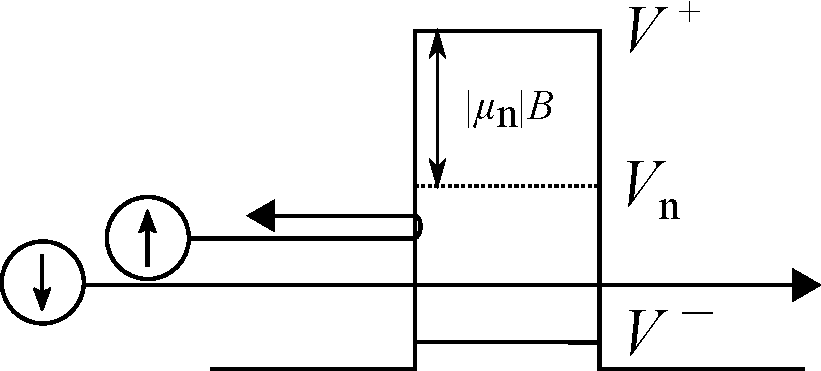
\includegraphics[width=8cm]{mirror/mono_mirror.pdf}
\caption{単層膜によるスピンの選択の原理。実際には、ポテンシャルは紙面奥に向かって2次元に広がっており、
中性子は臨界角以下で入射していることに注意。}
\end{figure}
このようにして、単層膜は上向きスピンの粒子のみを選択的に反射する。

\subsection{スーパーミラー}
\begin{figure}[H]
\centering
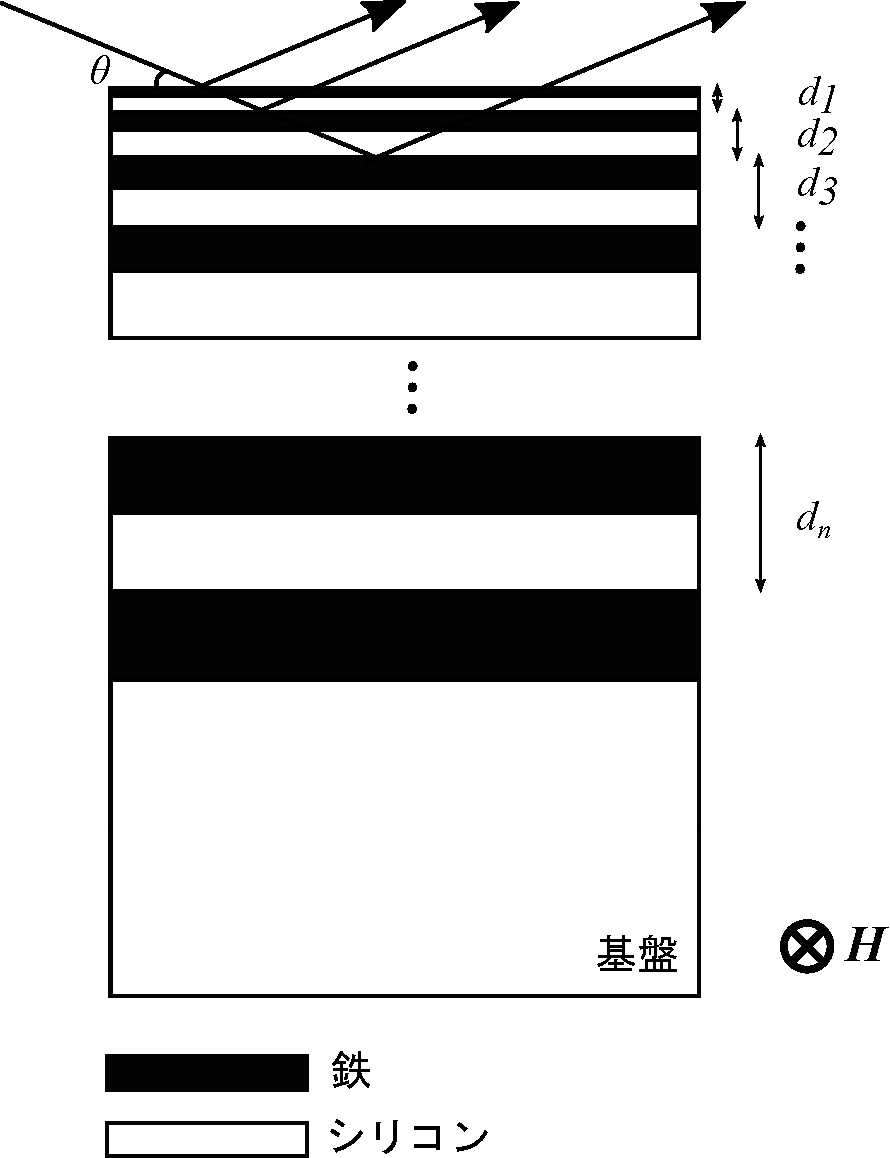
\includegraphics{mirror/super_mirror.pdf}
\caption{スーパーミラーの構造\cite{seki}\label{mirror_super_mirror}}
\end{figure}
\begin{figure}[h]
\centering
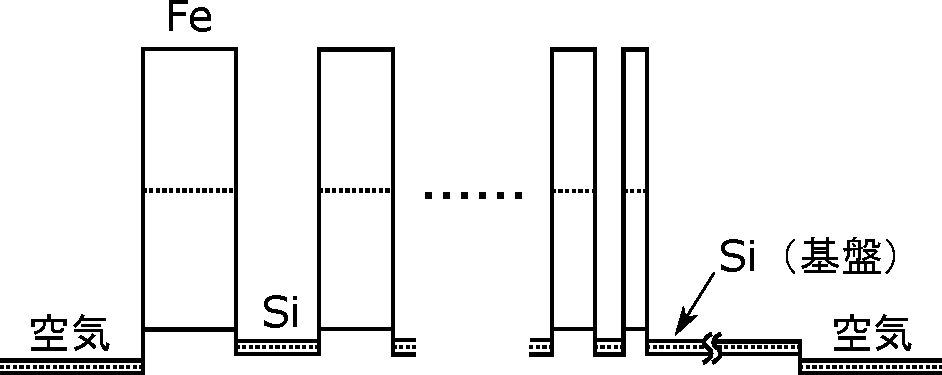
\includegraphics[width=9cm]{mirror/super_mirror_potential.pdf}
\caption{スーパーミラーのポテンシャル。破線は磁場によらない核力によるポテンシャル。実線(上)は上向きスピンの中性子が感じるポテンシャル。
実線(下)は下向きスピンの中性子が感じるポテンシャル。空気やシリコンの透磁率は小さいため、全体に磁場をかけても
ポテンシャルはほとんど影響を受けない。}
\end{figure}
図\ref{mirror_super_mirror}のように膜厚を少しずつ変えた多層膜を使うことで、
単層膜よりも高いエネルギーの中性子を反射するミラーを作ることができる。
これをスーパーミラーと呼ぶ。

\paragraph{Bragg反射による偏極}
$E\sin^2\theta\leq V^+$の中性子は多層膜の表面で全反射されるが、$V^+<E\sin^2\theta$の中性子は多層膜の内部に侵入する。
多層膜の膜間隔を$d$とすると、侵入した中性子はBragg条件
\begin{align}
2d\sin\theta=\lambda
\end{align}
を満たす場合に反射波が強め合う。$\lambda$は中性子の物質波の波長で、
$\lambda=2\pi/k$の関係にある。

$d$を少しずつ変えることで、$V^+<E\sin^2\theta$の様々なエネルギーを持つ上向きスピンの中性子がBragg反射される。
下向きスピンの中性子もわずかに反射されるが、その数は少なく、無視できる。
こうすることで、単層膜に比べより広いエネルギーの中性子のスピンを偏極することができる。

\section{検出器}
中性子は電荷をもたないため、その検出は強い相互作用を通じて行われる。強い相互作用による反応で生じた荷電粒子を検出することで、間接的に中性子を検出する。検出に利用する反応は検出する中性子のエネルギーによって様々であるが、熱中性子($\sim 25$ meV)の場合、次のような中性子捕獲反応が主に利用される:
\begin{align}
&\ce{^3He} + \ce{n} \to \ce{^3H}+\ce{p} + 0.705 \mathrm{MeV} \label{Kasuya_3He} \\
&\ce{^6Li} + \ce{n} \to \ce{^3H}+\ce{^4He}+4.78 \mathrm{MeV} \label{Kasuya_6Li}
\end{align}

\subsection{$\ce{^3He}$ガスを充填した比例計数管}
今回の実験では入射する中性子の時間情報と個数を知る必要がある。そこで入射粒子の数を1つずつ数える微分型の検出器として、$\ce{^3He}$ガスを充填した比例計数管を用いた。

\paragraph{検出原理}
検出には(\ref{Kasuya_3He})の反応が利用される。反応で生じた荷電粒子が気体中を進むと、軌道上の気体分子が電離してイオン・電子対が生じる。電場をかけてそれらを集めることで、信号として読み取ることができる。エネルギー25meVの中性子に対する$\ce{^3He}$原子核の断面積は$5333$barn[]であり、低エネルギーでこの断面積は中性子の速度に反比例することが知られている[]ため、エネルギー$E$(meV)の中性子に対する$\ce{^3He}$原子核の断面積は$\sigma(E)=5333\sqrt{25/E}$(barn)となる。これは気体の中では非常に大きく、効率よく中性子の数を数えることができる。

\paragraph{検出器の仕組み}
円筒形の容器の中に$\ce{^3He}$ガスが封入されており、高電圧がかけられた中心のワイヤと接地された容器の内壁がそれぞれ陽極と陰極として機能する。$\ce{^3He}$ガスは(\ref{Kasuya_3He})の反応によって荷電粒子を発生させる中性子有感物質であると共に、この荷電粒子によって電離して信号を増幅させる被電離気体の役割を果たす。

\begin{figure}[h]
\begin{minipage}{0.5\hsize}
\begin{center}
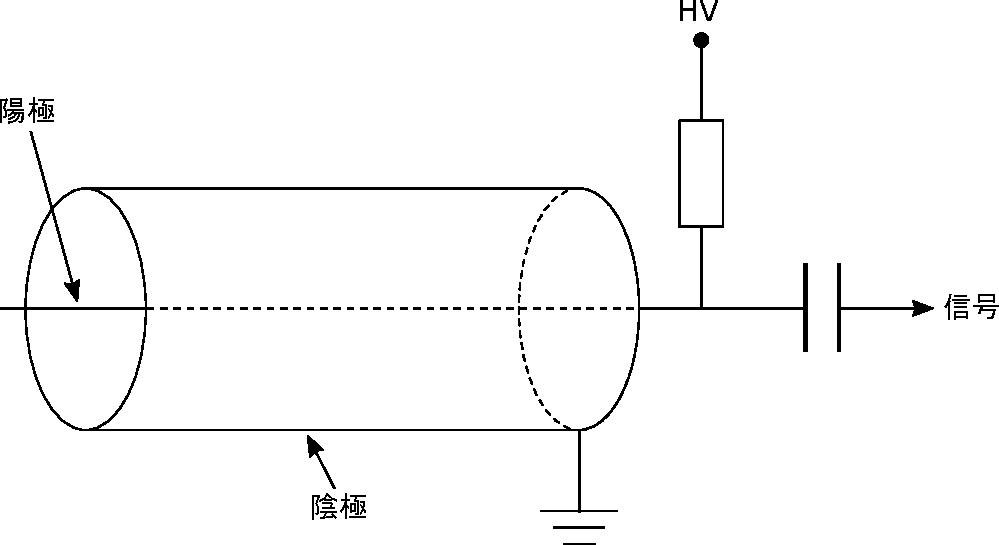
\includegraphics[width=6.5cm]{detector/detector_fig1.pdf}
\caption{比例計数管写真}
\end{center}
\end{minipage}
\begin{minipage}{0.5\hsize}
\begin{center}
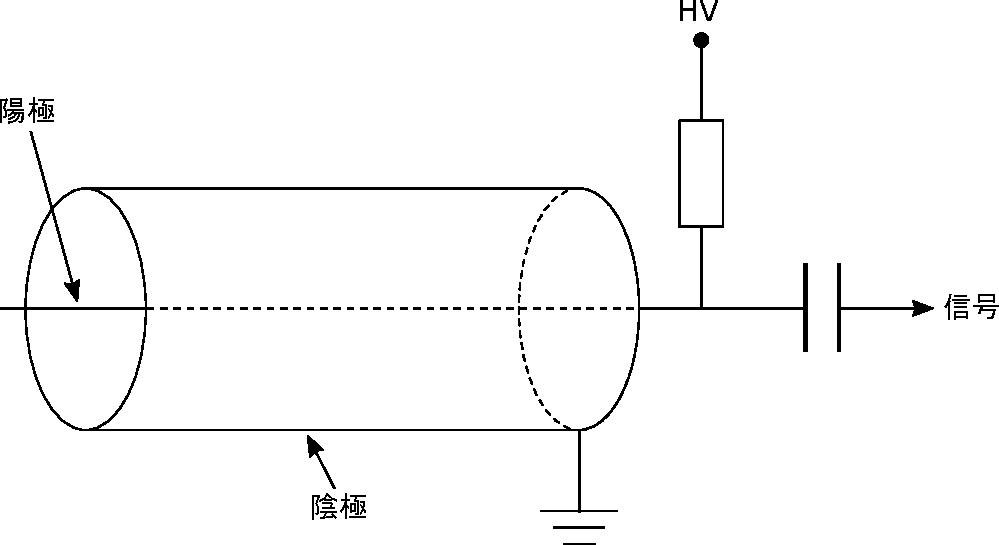
\includegraphics[width=6.5cm]{detector/detector_fig1.pdf}
\caption{比例計数管模式図}
\end{center}
\end{minipage}
\end{figure}

\subsection{RPMT検出器}
予備実験では入射する中性子の2次元的な位置情報を知る必要がある。そこで2次元位置感度型検出器として、RPMT検出器を用いた。

\paragraph{検出原理}
検出には(\ref{Kasuya_6Li})の反応が利用される。反応で生じた荷電粒子によってシンチレータ中の原子や分子が励起され、下の準位に戻る際に光が放出される(シンチレーション光)。生じた光は光電子増倍管で増幅され信号として取り出される。RPMTではシンチレータに$\ce{^6LiF}/\ce{ZnS}$を用いる。$\ce{^6LiF}/\ce{ZnS}$は発光量が大きくガンマ線感度が低いことから、中性子の検出に適している。

\paragraph{検出器の仕組み}
RPMTは$\ce{^6LiF}/\ce{ZnS}$シンチレータにPSPMT(Position Sensitive PMT,位置分解能をもつ光電子増倍管)を取り付けた構造をしている。PSPMTは内部にX軸Y軸のメッシュ状の読み取り用電極をもち、電荷分割法により中性子の検出位置を$x/L=Q_2/(Q_1+Q_2)$で求めることができる。ここで$L$は電極の全長、$x$は検出位置、$Q_1,Q_2$は2本のケーブルからの出力電荷である。検出位置はX軸Y軸について1024ch$\times$1024chの分解能で計測され、チャンネル幅[mm/ch]は$1\mathrm{[ch]}=0.119\pm0.002\mathrm{[mm]}$と報告されている[]。

\begin{figure}[h]
\begin{minipage}{0.5\hsize}
\begin{center}
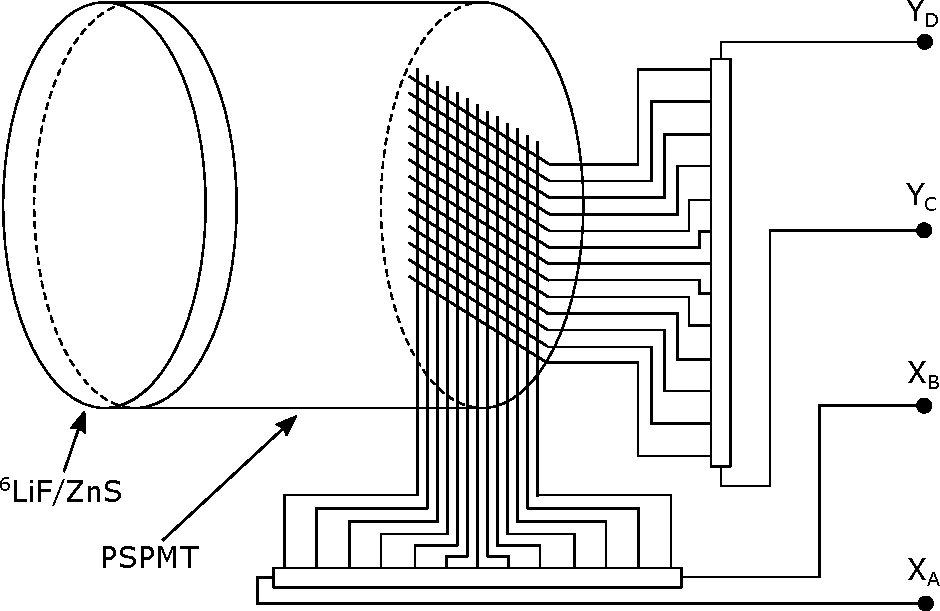
\includegraphics[width=6.5cm]{detector/detector_fig2.pdf}
\caption{RPMT写真}
\end{center}
\end{minipage}
\begin{minipage}{0.5\hsize}
\begin{center}
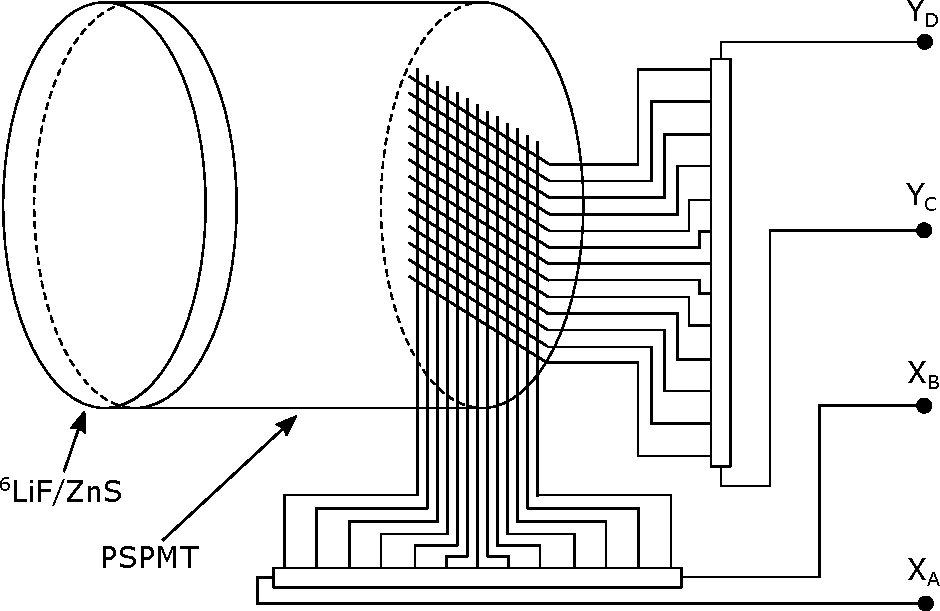
\includegraphics[width=6.5cm]{detector/detector_fig2.pdf}
\caption{RPMT模式図}
\end{center}
\end{minipage}\\
\begin{minipage}{0.5\hsize}
\begin{center}
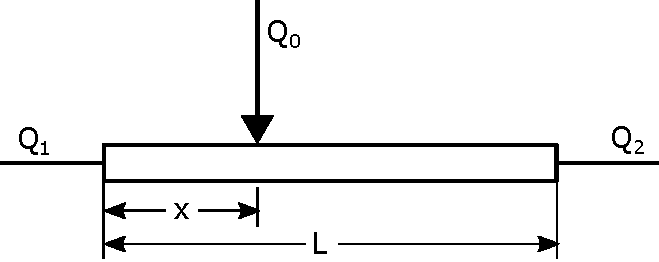
\includegraphics[width=6.5cm]{detector/detector_fig3.pdf}
\caption{電荷分割法}
\end{center}
\end{minipage}
\end{figure}






\section{予備実験:スピンフリッパーの共鳴}\label{resonance_sec}

「共鳴」は物理の様々な場所で登場する。例えば音叉の共鳴。固有振動数の等しいふたつの音叉を用意し片方だけを鳴らす。するともう一方もひとりでに鳴り始める。固有振動数の異なる音叉ではこのような現象は起こらない。このように、系がある特定の振動数に対してのみ特異なふるまいをみせる現象を、物理では広く「共鳴」と呼ぶ。

%スピンフリッパーの共鳴とは、フリッパーで特定の周波数の振動磁場をかけたときにフリッパーを通り抜けたある速度の中性子のスピンが完全に反転してしまう現象をいう。本実験における干渉パターンの見えやすさを高めるために、スピンフリッパーの共鳴が必要となる。
ではスピンフリッパーの共鳴とはいったい何だろうか。何のために共鳴させるのだろう。その実現方法は。この章ではそれらについて説明した後、実際の実験で用いた装置と従った手順、得られたデータを示し、最後にデータの分析を行う。

\subsection{What?\ $\sim$スピンフリッパーの共鳴とは何か$\sim$} \label{Resonance_what}
共鳴条件(\ref{pi2flipper_resonance})が満たされるとき、スピンフリッパーは共鳴しているという。その背後にどんな物理的意味が潜んでいるのだろうか。

一様磁場中に理想化されたRFスピンフリッパーがひとつ置かれた状況を考える。系は3つの領域I,II,IIIからなり、全体に$z$方向一様磁場$B_z$が、領域IIに$x$方向振動磁場$2B_r \cos \omega_s t$がかけられている。
\begin{figure}[h]
\centering
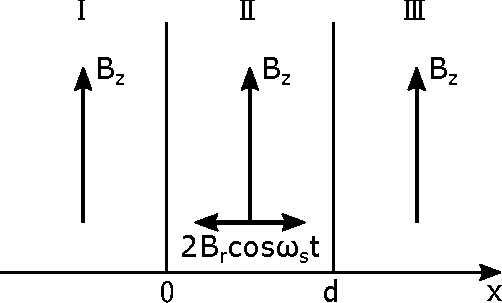
\includegraphics[height=3cm]{resonance/whatwhyhow/Resonance_what_setting.pdf}
\end{figure}

\ref{nonreso_sec}章で述べたように、領域Iからスピン上向きの中性子を入射したとき領域IIIでスピン上向きの中性子を観測する確率は
\begin{equation}
|\psi_{\mathrm{III}}^+|^2=\cos^2 \frac{\omega_A}{v}d+\left(\frac{\epsilon}{\omega_A}\right)^2\sin^2\frac{\omega_A}{v}d \label{Resonance_flip}
\end{equation}
となる。ここで$\epsilon=\omega_s/2-\omega_z,\omega_A=\sqrt{\epsilon^2+\omega_r^2}$であり、$\omega_z=|\mu_n|B_z,\omega_r=|\mu_n|B_r$、$\mu_n$は中性子の磁気モーメント、$d$は領域IIの幅である。

いま$\epsilon/|\omega_z|=0,0.3,0.5,1.0$の各場合についてスピンフリッパーを通過した中性子のスピン反転率($=1-|\psi_\mathrm{III}^+|^2$)と$\omega_r d/v$の関係を図\ref{Resonance_fig_reversalrate}に表す。
図\ref{Resonance_fig_reversalrate}より
\begin{equation}
\epsilon=\frac{\omega_s}{2}-\omega_z=0 \label{Resonance_resonance}
\end{equation}
がなりたてば、
\begin{equation}
\frac{\omega_r}{v}d =\frac{(2n+1)\pi}{2} \quad (n =0,1,2,\cdots) \label{Resonance_piflip_r}
\end{equation}
を満たす速度の中性子に対して、領域IIIにおけるスピン上向き粒子の存在確率が0、すなわちスピン反転率が1になることがわかる。逆に$\epsilon \neq 0$のときはどのような速度の中性子に対しても反転率は1となり得ない。このように、式(\ref{Resonance_resonance})を満たす周波数の振動磁場をかけたときに限りスピンフリッパーを通り抜けた中性子のスピンが完全に反転し得る。これをスピンフリッパーの共鳴と呼び、式(\ref{Resonance_resonance})を共鳴条件と呼ぶ。また速度に対する条件(\ref{Resonance_piflip_r})を$\pi$フリップ条件と呼ぶ。
\begin{figure}[h]
\begin{center}
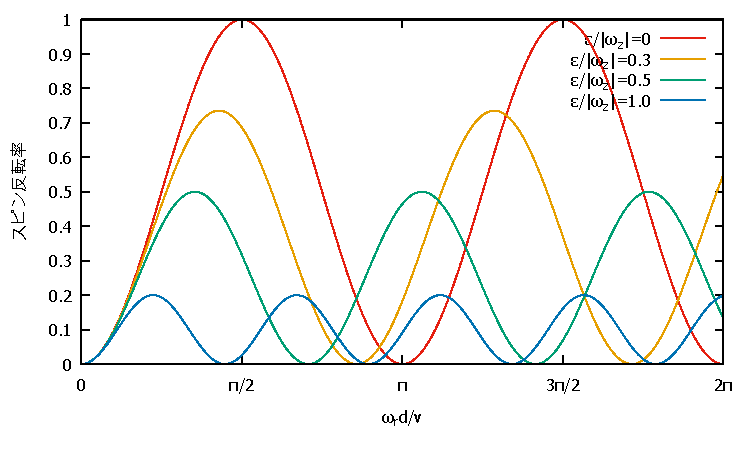
\includegraphics[width=9.5cm]{resonance/whatwhyhow/resonance_reversalrate.pdf}
\caption{スピン反転率}
\label{Resonance_fig_reversalrate}
\end{center}
\vspace{-1cm}
\end{figure}

\subsection{Why?\ $\sim$スピンフリッパーの共鳴はなぜ必要か$\sim$}
スピンフリッパーの共鳴は本実験での干渉がはっきり見えるかどうかの鍵を握っている。ここではスピンフリッパー共鳴の重要性が明らかとなる。

一様磁場中に、理想化されたRFスピンフリッパーふたつとシフタコイルひとつが置かれた状況を考える。系は7つの領域I,II,III,IV,V,VI,VIIからなり、全体に$z$方向一様磁場$B_z$がかけられ、それに加えて領域II,VIに$x$方向振動磁場$2B_r\cos\omega_s t$が、領域IVに$z$方向一様磁場$B$がかけられている。
\begin{figure}[h]
\centering
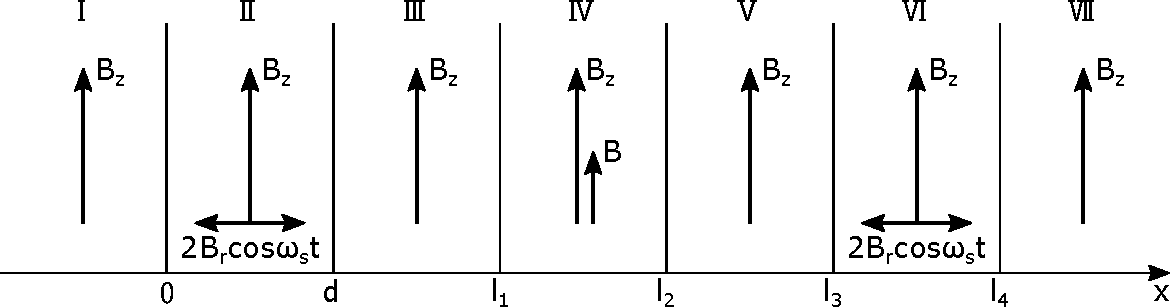
\includegraphics[height=3cm]{resonance/whatwhyhow/Resonance_why_setting.pdf}
\end{figure}

\ref{nonreso_sec}章で述べたように、スピン上向きの中性子が領域Iから入射し、領域I$\sim$VIを通って領域VIIに抜けるとき、領域VIIにおいてスピン上向き中性子を観測する確率は、共鳴からのずれを表すパラメータ$\epsilon$と中性子の速度$v$に依存した係数$N_1,N_2,N_3$を用いて
\begin{equation}
I=N_1-N_2\cos\left(\frac{2}{v}(\omega d'-\epsilon L')\right) -N_3\sin\left(\frac{2}{v}(\omega d'-\epsilon L')\right)
\end{equation}
と表せる。ここで$\omega$は位相シフタコイルの磁場$B$を用いて$\omega=|\mu_n|B$と表される量であり、$d',L'$はそれぞれ位相シフタコイルの幅、2つのスピンフリッパー間距離である。さらに$N_4=\sqrt{N_2^2+N_3^2}$として
\begin{equation}
\cos \phi=\frac{N_2}{N_4}, \quad \sin \phi=\frac{N_3}{N_4}
\end{equation}
で$\phi$を定義すれば、干渉パターンは
\begin{equation}
I=N_1-N_4\cos\left(\frac{2}{v}(\omega d'-\epsilon L')-\phi\right)\label{Resonance_interference}
\end{equation}
と書き直される。

いま、ある$\epsilon$に対して、シフタコイルの磁場を変えながら領域VIIでのスピン上向き中性子の数を計測すると式(\ref{Resonance_interference})の干渉パターンが得られるが、その見えやすさ(ビジビリティ)は$\epsilon$によって異なる。例えば$N_4/N1=1$のときは振幅の大きなはっきりとした(ビジビリティの高い)干渉パターンが得られるが、$N_4/N_1 \ll 1$のときは干渉パターンはほとんど観測できない(ビジビリティが低い)。そこでビジビリティを表す指標$V$を
\begin{equation}
V=\frac{N_4}{N_1}
\end{equation}
で定義すると、$0 \le V \le 1$であり、$V$が大きい程ビジビリティが高い。

いま$\epsilon/|\omega_z|=0,0.3,0.5,1.0$の各場合について干渉パターンのビジビリティ$V$と$\omega_r d/v$の関係を図\ref{Resonance_fig_visivility}に表す。図\ref{Resonance_fig_visivility}より共鳴条件(\ref{Resonance_resonance})がなりたてば、
\begin{equation}
\frac{\omega_r }{v}d =\frac{(2n+1)\pi}{4} \quad (n =0,1,2,\cdots) \label{Resonance_pi2flip_r}
\end{equation}
を満たす速度の中性子に対して、干渉パターンのビジビリティ$V=1$になることがわかる。逆に$\epsilon \neq 0$のときはどのような速度の中性子に対してもビジビリティは1となり得ない。この速度に対する条件(\ref{Resonance_pi2flip_r})を$\pi/2$フリップ条件と呼ぶ。実際、$\omega_rd/v=\pi/4$,$\epsilon/|\omega_z|=0,0.3,0.5,1.0$のときの干渉パターンは図\ref{Resonance_fig_interference}のようになる。すなわちスピンフリッパーを共鳴させる目的は、本実験で得られる干渉パターンのビジビリティを高めるためである。

\begin{figure}[h]
\vspace{-2mm}
\begin{center}
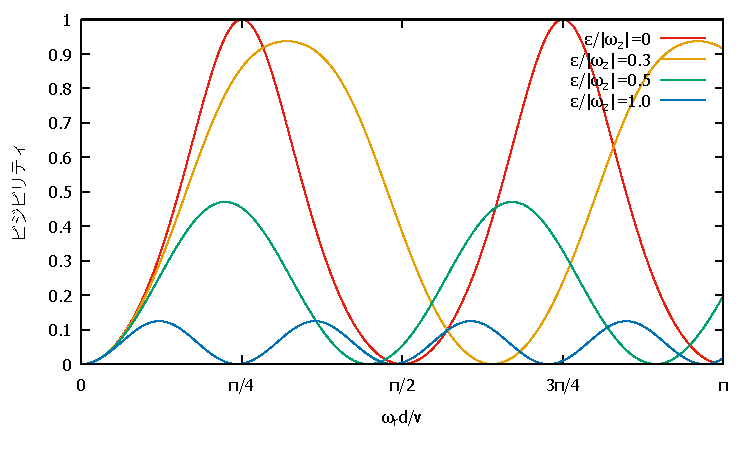
\includegraphics[width=9.5cm]{resonance/whatwhyhow/resonance_visivility1.pdf}
\caption{ビジビリティ}
\label{Resonance_fig_visivility}
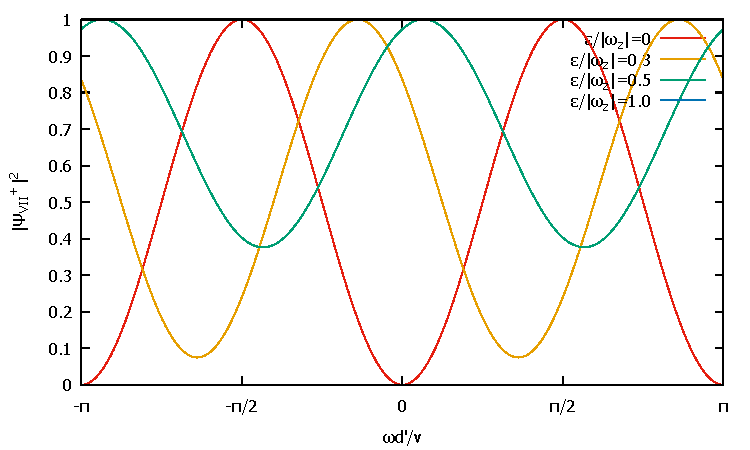
\includegraphics[width=9.5cm]{resonance/whatwhyhow/resonance_interference1.pdf}
\caption{干渉パターン}
\label{Resonance_fig_interference}
\end{center}
\vspace{-1cm}
\end{figure}



\clearpage
\subsection{How?\ $\sim$スピンフリッパーを共鳴させるには$\sim$}
実際にスピンフリッパーを共鳴させるにはどうしたらよいだろう。ここではその実現方法を考え、実際に実験で用いた装置と従った手順を紹介する。

\paragraph{実現方法}
\ref{Resonance_what}節と同じく、一様磁場中にスピンフリッパーがひとつ置かれており、スピン上向き中性子を領域Iから入射させる場合を考える。このとき領域IIIでスピン上向き中性子を観測する確率は式(\ref{Resonance_flip})より
\begin{equation}
|\psi_\mathrm{III}^+|^2 =\cos^2 \frac{\omega_A}{v}d+\left(\frac{\epsilon}{\omega_A}\right)^2\sin^2\frac{\omega_A}{v}d
\end{equation}
であらわされる。これを$\omega_r/|\omega_z|=0.5$のときに、$\epsilon/|\omega_z|=0,0.3,0.5,1.0$の各場合について$\omega_r d/v$に対して図示すると図\ref{Resonance_fig_1-reversal}のようになる。図\ref{Resonance_fig_1-reversal}より、領域IIIでスピン上向き中性子を観測する確率の、速度に対する最小値は共鳴条件(\ref{Resonance_resonance})
を満たすとき最も小さくなり、理想的にはゼロとなることがわかる。共鳴条件を満たすときにスピンフリッパーを通り抜けた中性子のスピン反転率が$1,1/2$となるための中性子の速度に対する条件をそれぞれ$\pi$フリップ条件(\ref{Resonance_piflip})、$\pi/2$フリップ条件(\ref{Resonance_pi2flip})と呼んだが、今回の実験で用いた中性子の速度範囲ではそれぞれ$n=0$の場合のみが満たされ得るので、以後
\begin{equation}
\frac{\omega_r}{v}d=\frac{\pi}{2}\label{Resonance_piflip}
\end{equation}
を$\pi$フリップ条件
\begin{equation}
\frac{\omega_r}{v}d=\frac{\pi}{4}\label{Resonance_pi2flip}
\end{equation}
を$\pi/2$フリップ条件と呼ぶことにする。
\begin{figure}[h]
\begin{center}
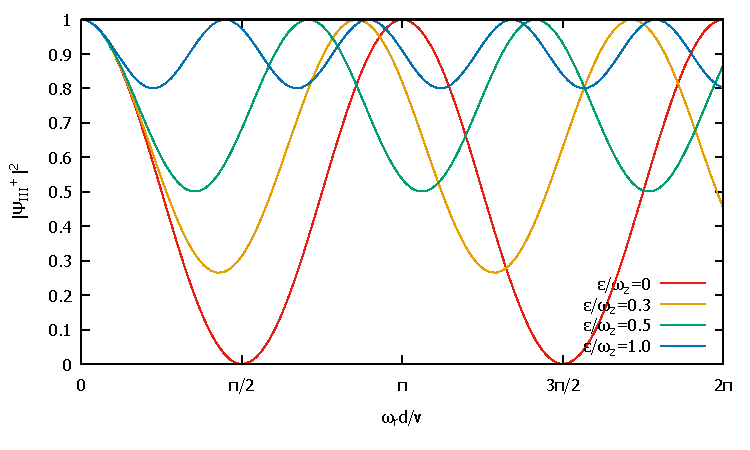
\includegraphics[width=9.5cm]{resonance/whatwhyhow/resonance_1-reversal.pdf}
\caption{$1-反転率$}
\label{Resonance_fig_1-reversal}
\end{center}
\end{figure}

すなわち次のようにして、実験的にスピンフリッパーの共鳴を実現することができる。
\begin{enumerate}
\item スピンフリッパーにスピン上向き中性子を入射し、フリッパーの後ろでスピン上向き成分のみを観測する。
\item 共鳴条件(\ref{Resonance_resonance})が満たされていないと、ある速度の中性子についてはカウントをより減らすことができる。
\item 共鳴条件(\ref{Resonance_resonance})が満たされていると、$\pi$フリップ条件(\ref{Resonance_piflip})を満たす速度の中性子についてはスピンが完全に反転するため、その速度の中性子のカウントは最小となる。
\item カウント分布を見ながら共鳴条件(\ref{Resonance_resonance})に関するパラメータを調節し、カウントが最小となるところを探す。
\end{enumerate}


\paragraph{実験装置}
上流側、下流側それぞれのスピンフリッパーに対して共鳴実験を行った。用いた装置は
\vspace{5mm}
\begin{minipage}{0.5\hsize}
\begin{enumerate}
\item 上流側スピンフリッパー共鳴実験
\begin{enumerate}
\item ガイド磁場コイル
\item 上流側中性子磁気スーパーミラー
\item[(c1)] 上流側スピンフリッパー
\setcounter{enumii}{3}
\item 下流側中性子磁気スーパーミラー
\item \ce{^3He}ガスを充填した比例計数管
\end{enumerate}
\end{enumerate}
\end{minipage}
\begin{minipage}{0.5\hsize}
\begin{enumerate}
\setcounter{enumi}{1}
%\renewcommand{\labelenumi}{}
\item 下流側スピンフリッパー共鳴実験
\begin{enumerate}
\item ガイド磁場コイル
\item 上流側中性子磁気スーパーミラー
%\renewcommand{\labelenumi}{(\alph{enumi} {2})}
\item[(c2)] 下流側スピンフリッパー
\setcounter{enumii}{3}
%\renewcommand{\labelenumi}{(\alph{enumi})}
\item 下流側中性子磁気スーパーミラー
\item \ce{^3He}ガスを充填した比例計数管
\end{enumerate}
\end{enumerate}
\end{minipage}
\vspace{5mm}

また、回路系には次の機器を用い、図のように接続した。
\begin{enumerate}
\renewcommand{\labelenumi}{(\roman{enumi})}
\item 直流安定化電源PWX750MLF(KIKUSUI) $\times 3$ \ \ (以後、直流電源1,2,3)
\item マルチファンクションジェネレータWF1974(エヌエフ回路設計ブロック) \ \ (以後、FG)
\item 1MHzバイポーラ電源HSA4014(エヌエフ回路設計ブロック) $\times 2$ \ \ (以後、アンプ1,2)
\end{enumerate}

\vspace{5mm}
\begin{figure}[h]
\centering
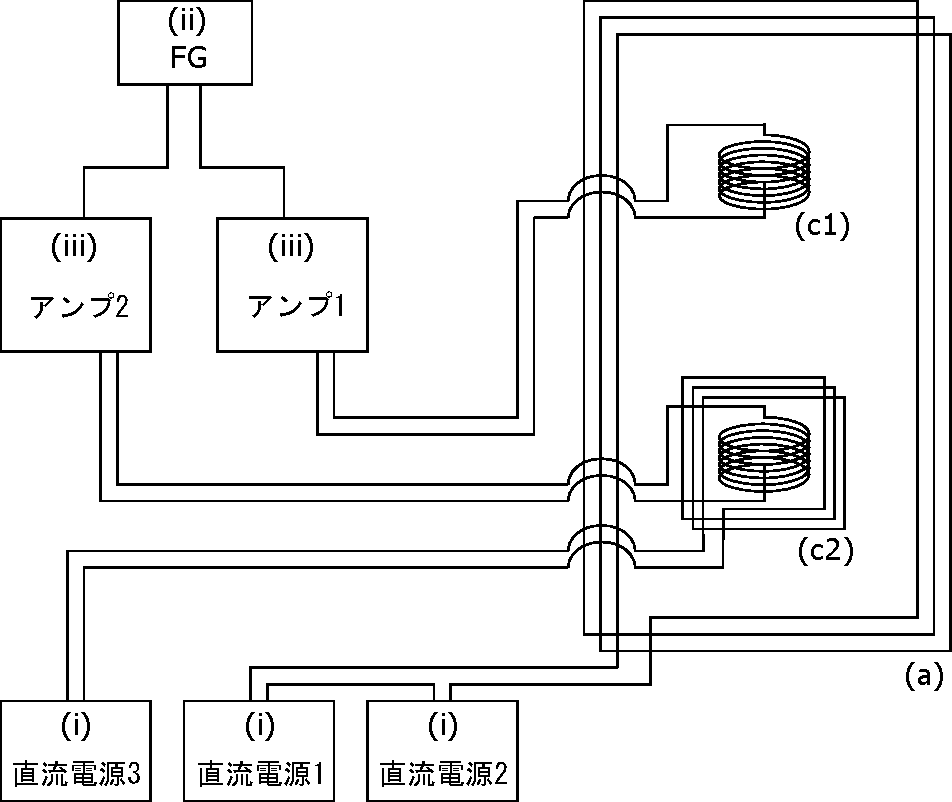
\includegraphics[width=12cm]{resonance/whatwhyhow/kairozu.pdf}
\caption{配線図}
\vspace{-5mm}
\end{figure}

\clearpage
\paragraph{実験手順}
実験は次のフローチャートに沿って行った。
\begin{figure}[h]
\centering
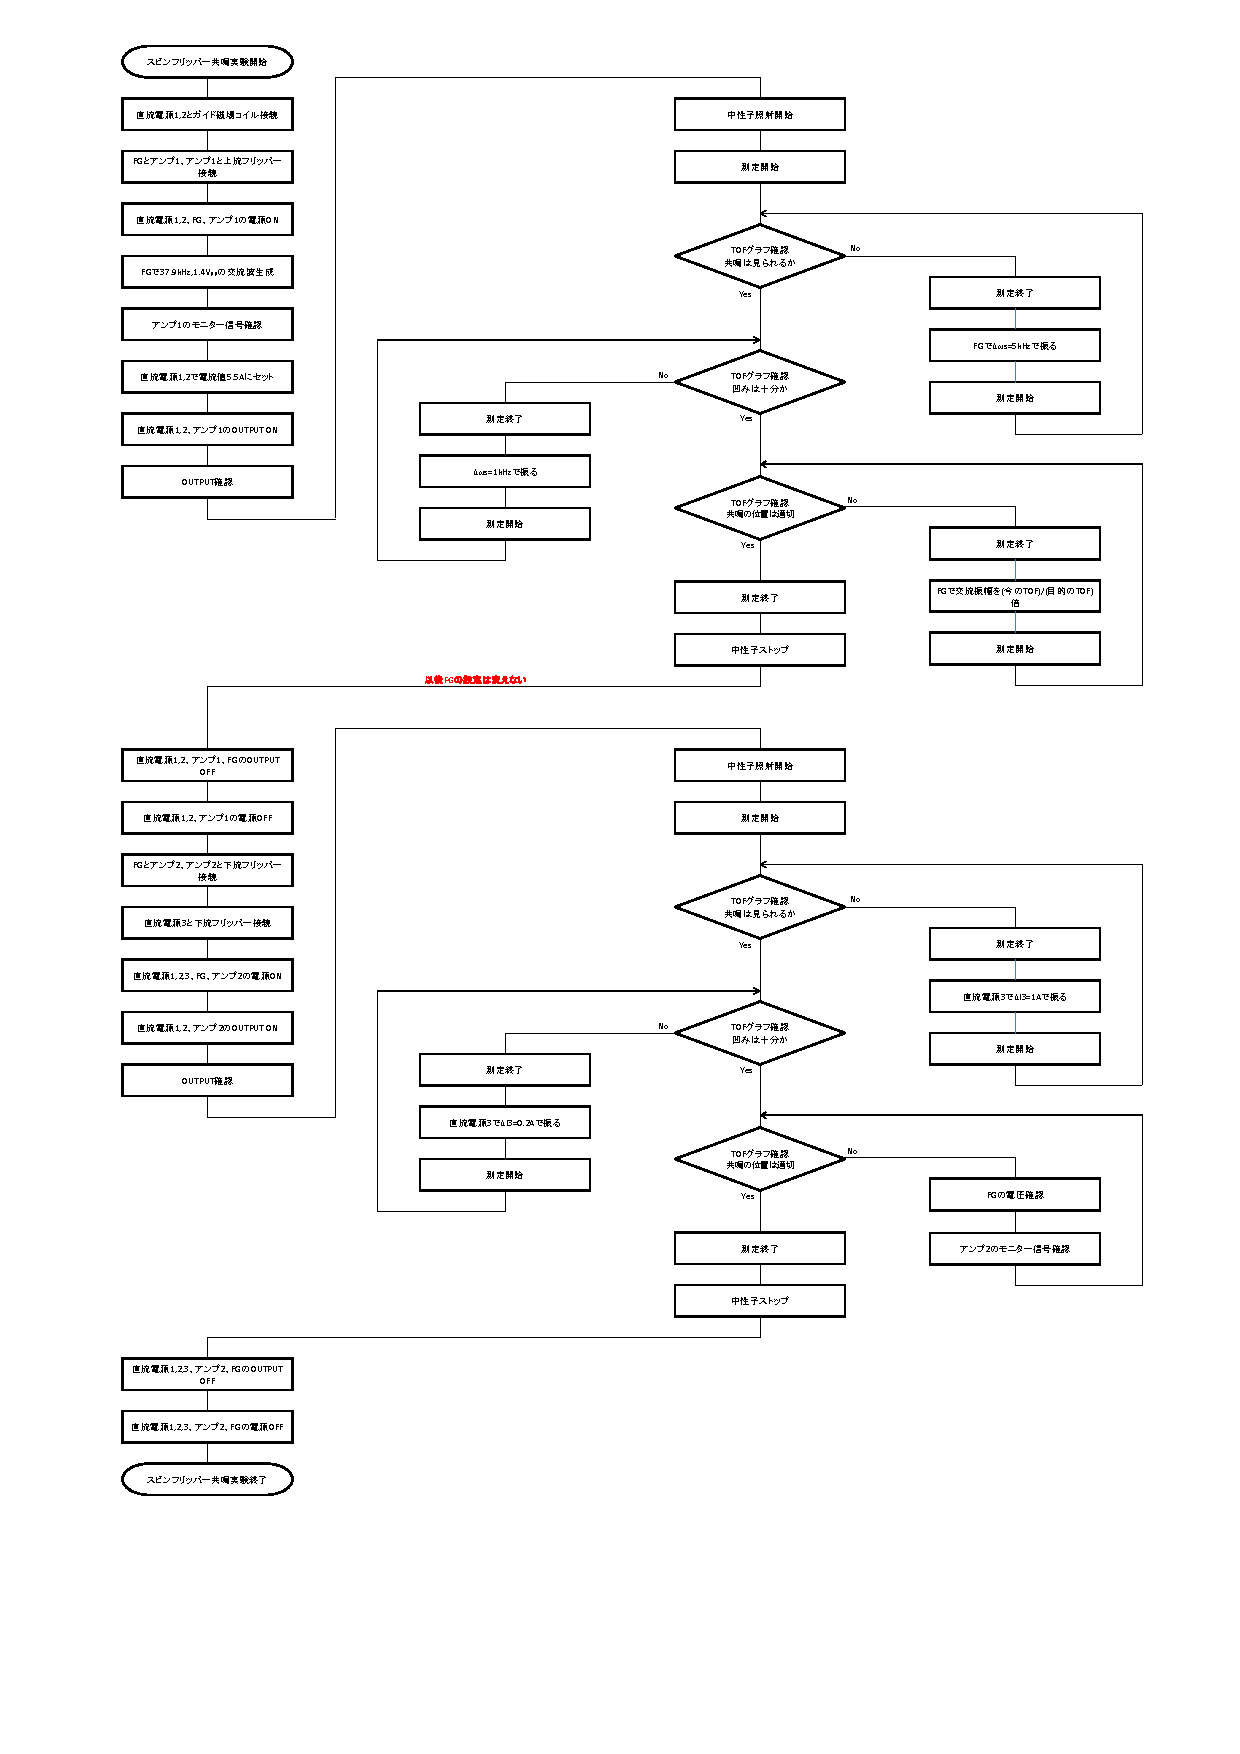
\includegraphics[width=\hsize]{resonance/whatwhyhow/Resonance_flow.pdf}
\vspace{-3.5cm}
\end{figure}

\newpage
次は実際の実験手順である。
\begin{enumerate}
%\renewcommand{\labelenumi}{\arabic{enumi})}
\item (2017.2.22)装置、機器を図のとおりに配置、接続し、上流フリッパー共鳴実験を開始した。
\item 直流電源1,2でガイド磁場コイルに5.5Aの電流を流した。
\item FGで周波数$37.9\, \mathrm{kHz},振幅14.0\, \mathrm{V_{pp}}$の交流波を生成し、アンプ1で増幅して上流フリッパーに交流電流を流した。
\item 中性子の照射を開始した。
\item 測定を開始した。
\item 10分程度データを取り、TOF分布に凹みを確認した。
\item FGで交流波の周波数を$37.0,38.8,36.0,34.0,41.0,40.0 \, \mathrm{kHz}$と変えながら、それぞれ10分程度データを収集した。
\item データ収集と平行して解析を行い、交流波の周波数を$37.5\, \mathrm{kHz}$,振幅を$14.0\, \mathrm{V_{pp}}$に決定した。
\item 中性子照射をストップし、機器の電源を落として上流フリッパー共鳴実験を終了した。
\item (2017.2.23)装置、機器を図のとおりに配置、接続し、下流フリッパー共鳴実験を開始した。
\item 直流電源1,2でガイド磁場コイルに5.5Aの電流を流した。
\item FGで周波数$37.5\, \mathrm{kHz},振幅14.0\, \mathrm{V_{pp}}$の交流波を生成し、アンプ2で増幅して下流フリッパーに交流電流を流した。
\item 中性子の照射を開始した。
\item 測定を開始した。
\item 10分程度データを取り、TOF分布に凹みを確認した。
\item 直流電源3でガイド磁場補正用コイルに流す電流を$0.1,0.5,0.3,0.7\,\mathrm{A}$と変えながら、それぞれ10分程度データを収集した。
\item 一旦中性子照射をストップし直流電源3をガイド磁場補正用コイルに逆向きにつなぎ替え、再び中性子照射を開始した。
\item 直流電源3でガイド磁場補正用コイルに流す電流を$-1.0,-0.5,-2.0\,\mathrm{A}$と変えながら、それぞれ10分程度データを収集した。
\item 一旦中性子照射をストップし直流電源3をガイド磁場補正用コイルに逆向きにつなぎ替え、再び中性子照射を開始した。
\item 直流電源3でガイド磁場補正用コイルに流す電流を$1.0,2.0\,\mathrm{A}$と変えて、それぞれ10分程度データを収集した。
\item データ収集と平行して解析を行い、ガイド磁場補正用コイルの電流値を$0.185\,\mathrm{A}$に決定した。
\item 中性子照射をストップし、機器の電源を落として下流フリッパー共鳴実験を終了した。
\end{enumerate}

\begin{itemize}
\item[(注$\!\!$1)] ガイド磁場コイル、ガイド磁場補正用コイルに流す電流は、電流を流したときに鉛直下向きの磁場が発生する向きを正とした。
\item[(注$\!\!$2)] 下流フリッパー共鳴実験中、ガイド磁場コイルが接触不良のためうまく機能せず正しいデータが取れない事態が発生したが、それについては省略した。
\end{itemize}

%\newpage
\paragraph{パラメータ初期設定}
スピンフリッパー共鳴実験で実際に制御できるパラメータはFGで生成する交流電圧の周波数$f_s$,振幅$V_r$と直流電源3で下流フリッパーのガイド磁場補正用コイルに流す電流$I_c$の3つである。実験は共鳴条件(\ref{Resonance_resonance})と$\pi$フリップ条件(\ref{Resonance_piflip})を満たすようにこれらを適当に変えながら進めたが、初期設定としてこれらの値をある程度正確に決めておく必要がある。なぜなら、もし最初に全く共鳴が見えないと、どのパラメータをどの程度動かしてよいか全く見当がつかないから。

スピンフリッパーにかける振動磁場の角振動数$\omega_s$と振幅$2B_r$の2つのは、それぞれフリッパーが置かれた場所におけるガイド磁場コイルの磁場$B_z$とターゲットとする中性子の速度$v$から定まる。すなわち$\omega_s$は共鳴条件(\ref{Resonance_resonance})より
\begin{equation}
\omega_s = 2\omega_z =2 |\mu_n|B_z
\end{equation}
$B_r$は$\pi$フリップ条件(\ref{Resonance_piflip})より
\begin{equation}
2B_r =\frac{2 \omega_r}{|\mu_n|} =\frac{\pi v}{|\mu_n|d}
\end{equation}
で定まる。

$B_z$としてはシミュレーションと実測より$B_z=-13 \, \mathrm{G}$を、$v$としてはフリッパー無しのときの速度分布である程度カウントの多かった$v=1000\, \mathrm{m/s}$を入れてそれぞれ計算すると
\begin{equation}
|\omega_s|/2\pi\simeq 37.9\, \mathrm{kHz}, \quad B_r\simeq 5.7 \, \mathrm{G}
\end{equation}
を得る。従ってFGで生成する交流電圧の周波数$f_s$の初期値は$37.9\,\mathrm{kHz}$と決めた。

また、フリッパーを直径90mm幅30mmの30巻きソレノイドコイルとして、1Aの電流を流したときの中心での磁場の大きさ$b_f$[G]と、37.9kHzの交流電圧をかけたときのインピーダンス$Z[\Omega]$を計算するとそれぞれ
\begin{equation}
b_f\simeq 3.9 \,\mathrm{G} \qquad Z \simeq 24.5 \,\Omega
\end{equation}
となる。ゆえにフリッパーにかける交流電圧の振幅(peak to peak)は
\[2 \times \frac{2B_r}{b_f} \times Z \simeq 140 \mathrm{V_{pp}}\]
となる。アンプで振幅を約100倍にすることを考えて、FGで生成する交流電圧の振幅$V_r$の初期値は$1.4 \,\mathrm{V_{pp}}$と決めた。

また、シミュレーションと実測よりガイド磁場の大きさは上流フリッパーの位置と下流フリッパーの位置でほぼ等しいことがわかっていたため、フリッパーのガイド磁場補正用コイルに流す電流の$I_c$の初期値は$0\,\mathrm{A}$と決めた。

まとめると
\begin{table}[h]
\centering
\caption{パラメータ初期値}
\begin{tabular}{ccc}
$f_s$の初期値&$V_r$の初期値&$I_c$の初期値 \\ \hline
$37.9\,\mathrm{kHz}$&$1.4 \,\mathrm{V_{pp}}$&$0\,\mathrm{A}$
\end{tabular}
\end{table}

\subsection{測定データ}
実際に共鳴実験で得られたデータを以下に示す。上流フリッパー共鳴実験で周波数を$|\omega_s|/2\pi=34.0,36.0,37.0,37.9,38.8,40.0,41.0$kHzと変えたとき、それぞれの場合に得られた粒子数の波長分布を図\ref{Resonance_fig_Flipper1_RawCounts}に、下流フリッパー共鳴実験でガイド磁場補正用コイル電流を$I_c=-2.0,-1.0,-0.5,0,0.1,0.3,0.5,1.0,2.0$Aと変えたとき、それぞれの場合に得られた粒子数の波長分布を図\ref{Resonance_fig_Flipper2_RawCounts}に表す。

\begin{figure}[h]
%\begin{minipage}{0.49\hsize}
%\centering
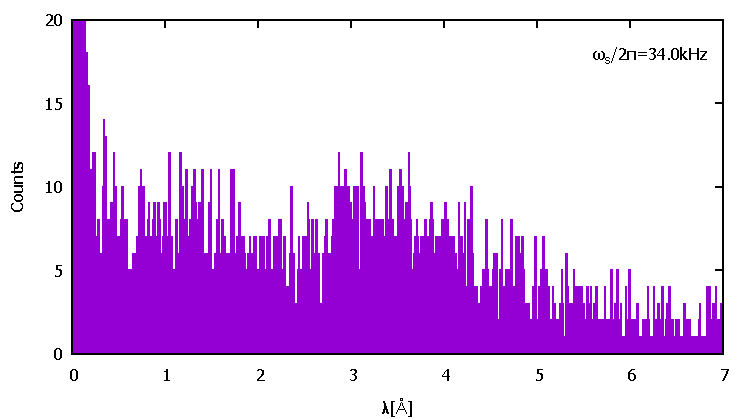
\includegraphics[height=4.3cm]{resonance/results/Flipper1_RawCounts_340kHz.pdf}
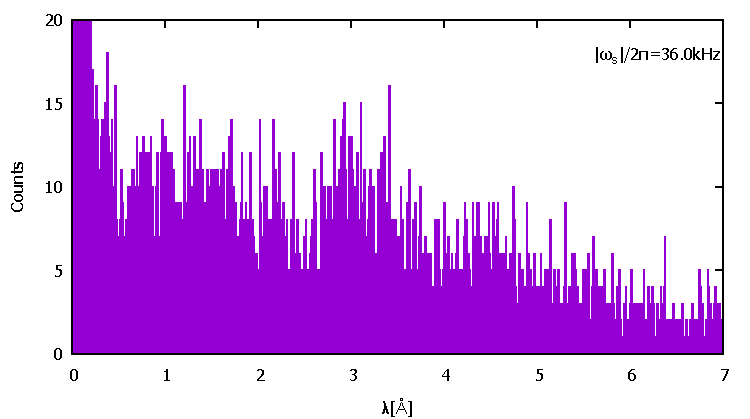
\includegraphics[height=4.3cm]{resonance/results/Flipper1_RawCounts_360kHz.pdf}\\
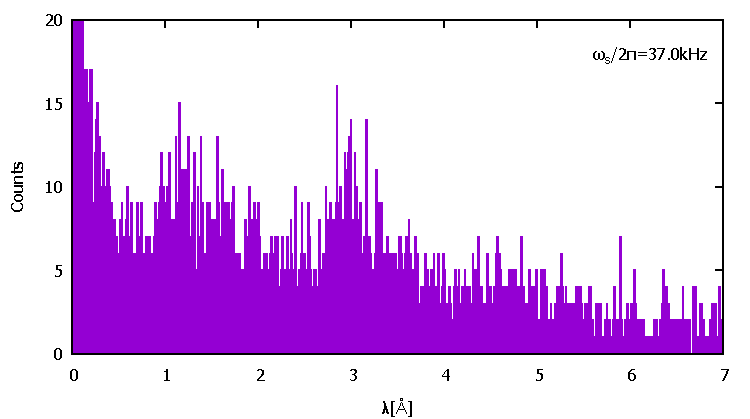
\includegraphics[height=4.3cm]{resonance/results/Flipper1_RawCounts_370kHz.pdf}
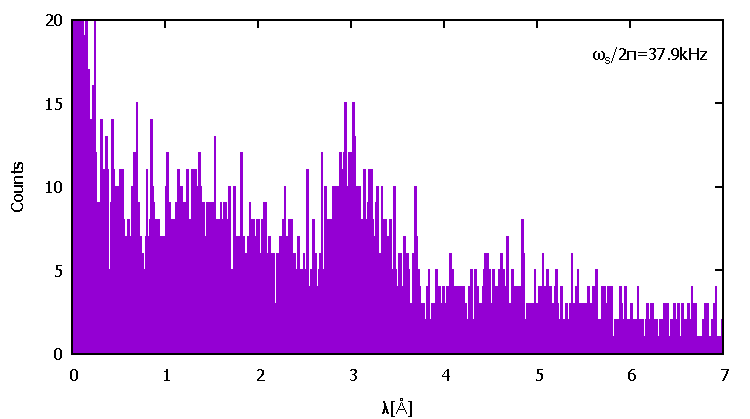
\includegraphics[height=4.3cm]{resonance/results/Flipper1_RawCounts_379kHz.pdf}\\
%\end{minipage}
%\begin{minipage}{0.49\hsize}
%\centering
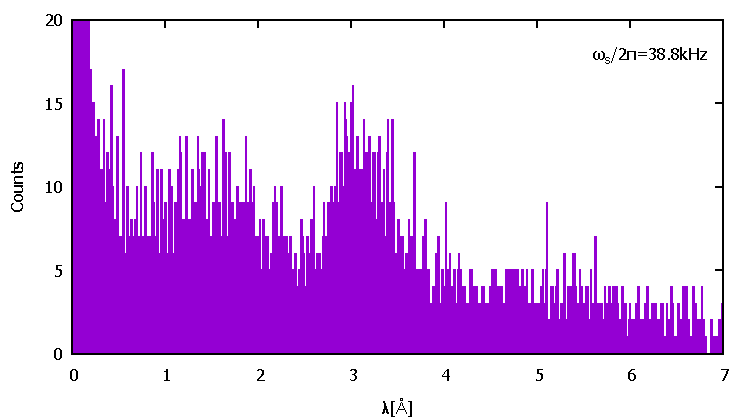
\includegraphics[height=4.3cm]{resonance/results/Flipper1_RawCounts_388kHz.pdf}
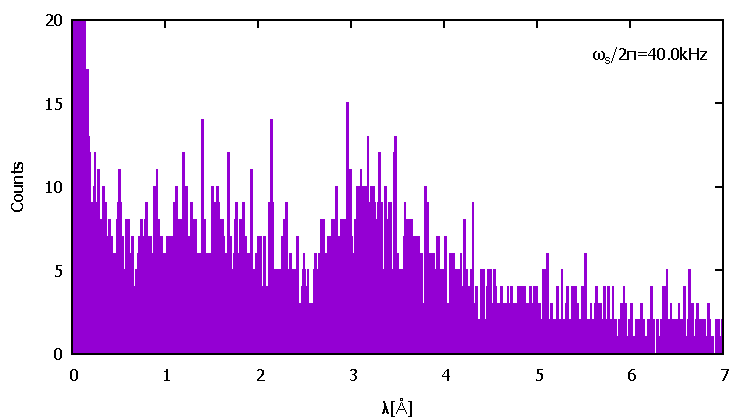
\includegraphics[height=4.3cm]{resonance/results/Flipper1_RawCounts_400kHz.pdf}\\
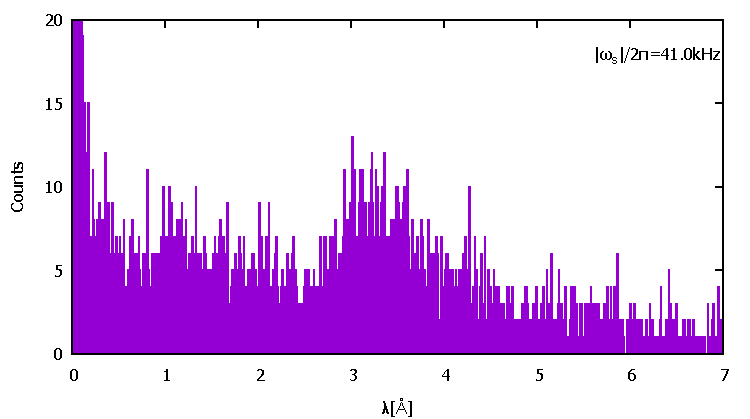
\includegraphics[height=4.3cm]{resonance/results/Flipper1_RawCounts_410kHz.pdf}
%\vspace{4.3cm}
%\end{minipage}
\caption{上流フリッパー共鳴実験で得られた粒子数の波長分布}\label{Resonance_fig_Flipper1_RawCounts}
\end{figure}

\begin{figure}[h]
%\begin{minipage}{0.5\hsize}
%\centering
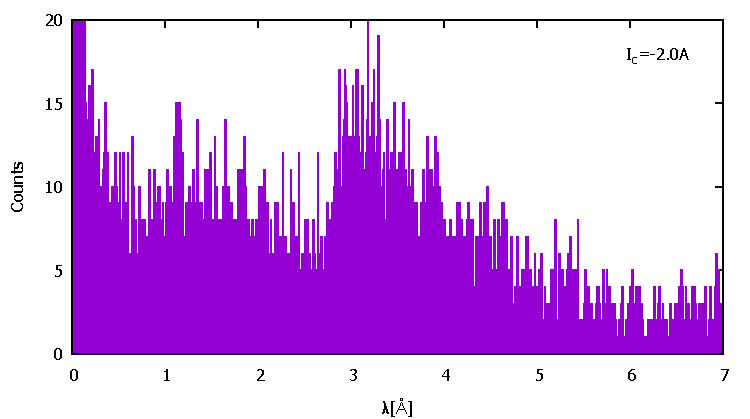
\includegraphics[height=4.3cm]{resonance/results/Flipper2_RawCounts_-20A.pdf}
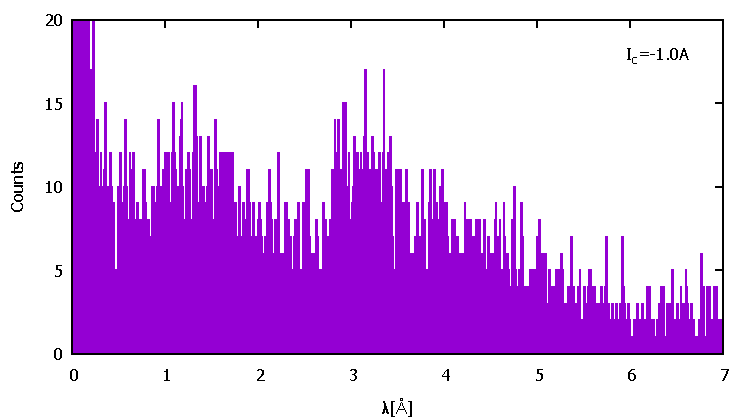
\includegraphics[height=4.3cm]{resonance/results/Flipper2_RawCounts_-10A.pdf}\\
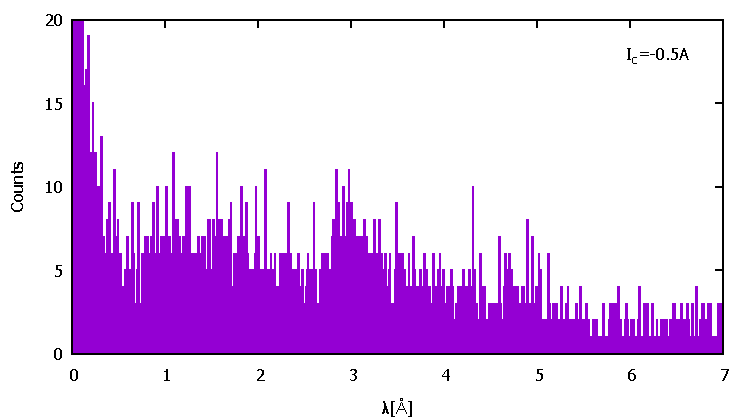
\includegraphics[height=4.3cm]{resonance/results/Flipper2_RawCounts_-5A.pdf}
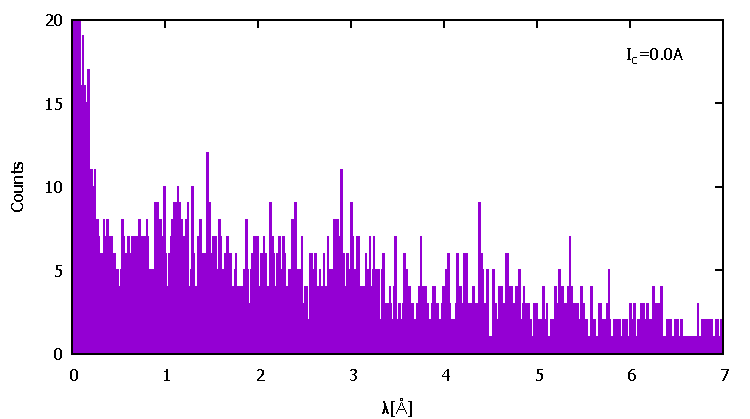
\includegraphics[height=4.3cm]{resonance/results/Flipper2_RawCounts_0A.pdf}\\
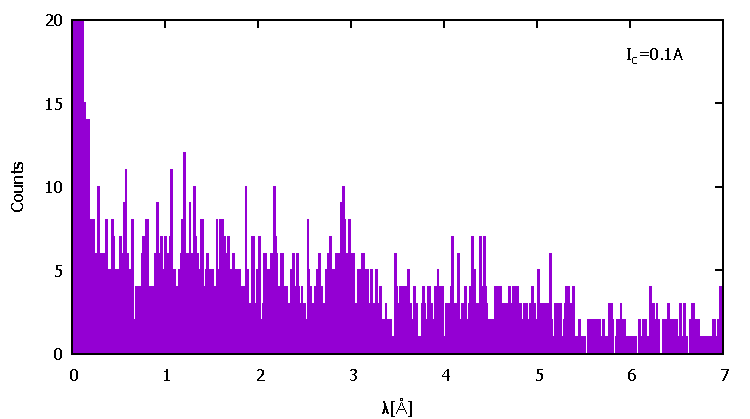
\includegraphics[height=4.3cm]{resonance/results/Flipper2_RawCounts_1A.pdf}
%\end{minipage}
%\begin{minipage}{0.5\hsize}
%\centering
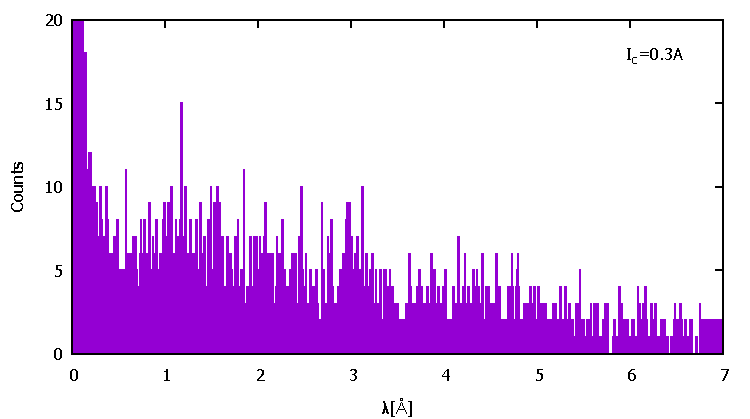
\includegraphics[height=4.3cm]{resonance/results/Flipper2_RawCounts_3A.pdf}\\
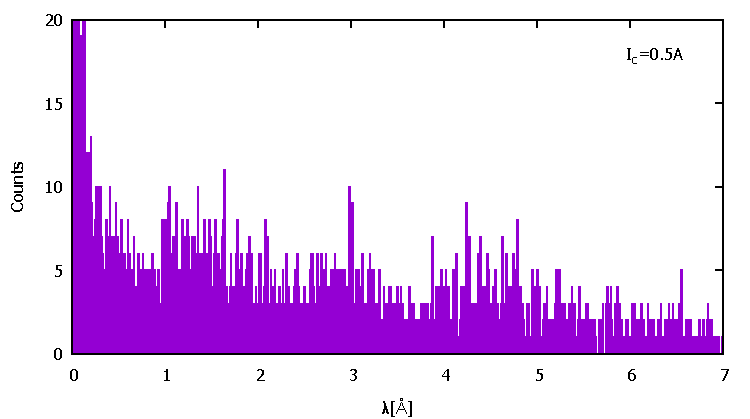
\includegraphics[height=4.3cm]{resonance/results/Flipper2_RawCounts_5A.pdf}
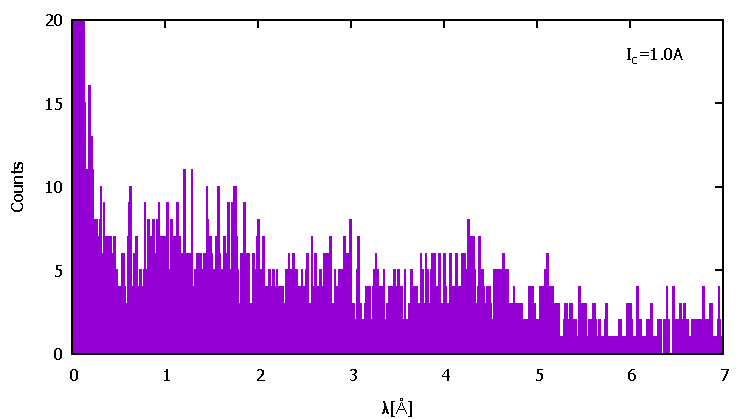
\includegraphics[height=4.3cm]{resonance/results/Flipper2_RawCounts_10A.pdf}\\
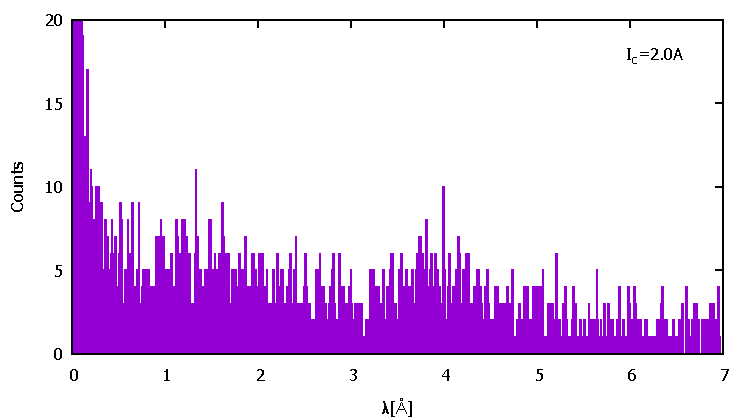
\includegraphics[height=4.3cm]{resonance/results/Flipper2_RawCounts_20A.pdf}
%\vspace{4.3cm}
%\end{minipage}
\caption{下流フリッパー共鳴実験で得られた粒子数の波長分布}\label{Resonance_fig_Flipper2_RawCounts}
\end{figure}

\clearpage
\subsection{分析}
以下では
\begin{enumerate}
\item 上流フリッパーについてデータから共鳴条件(\ref{Resonance_resonance})を満たす$\omega_s$を決め、グラフから共鳴時に最もよくスピン反転する中性子の波長を推定し、$\pi$フリップ条件(\ref{Resonance_piflip})から$\omega_r$を計算する。
\item 上流フリッパーについてデータから共鳴条件(\ref{Resonance_resonance})を満たす$I_c$を決め、グラフから共鳴時に最もよくスピン反転する中性子の波長を推定し、$\pi$フリップ条件(\ref{Resonance_piflip})から$\omega_r$を計算する。
\end{enumerate}
という流れでデータの分析を行う。

\paragraph{上流フリッパーに関する分析}
共鳴しているかを知るにはパラメータを変えたときの検出粒子数を比較すればよく、ある波長でカウントが最小となるとき共鳴していると考えてよい。しかし前節で示したデータは測定時間や加速器の出力がそれぞれ異なるので、そのままでは互いに比較することができない。そこで測定データのカウントをそのデータの測定開始時刻から測定終了時刻までにおけるLiMのカウントで割って規格化することで、データを互いに比較できるようにする。このようにして規格化した上流フリッパー共鳴実験における粒子数の波長分布を、フリッパーをOFFにしたときの規格化粒子数と共に、図\ref{Resonance_fig_Flipper1_NormalizedCounts}に表す。

\begin{figure}[h]
%\begin{minipage}{0.49\hsize}
%\centering
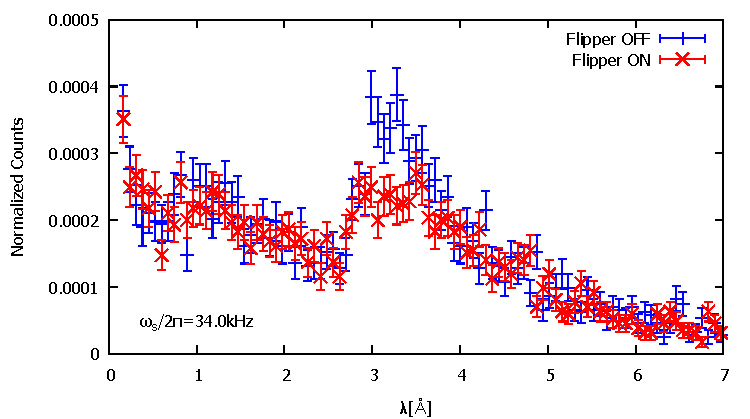
\includegraphics[height=4.3cm]{resonance/analysis/Flipper1_NormalizedCounts_340kHz.pdf}
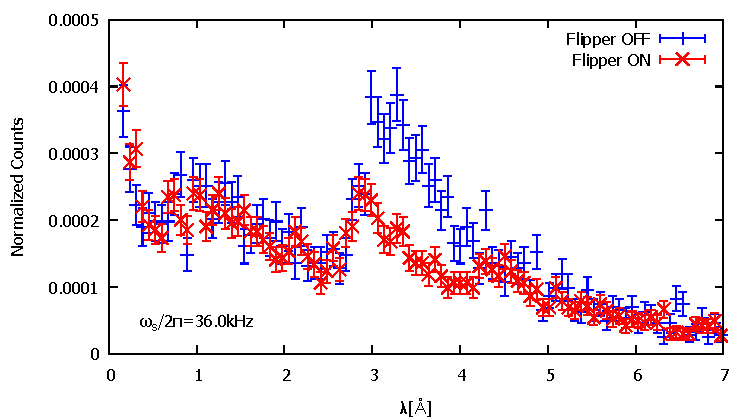
\includegraphics[height=4.3cm]{resonance/analysis/Flipper1_NormalizedCounts_360kHz.pdf}\\
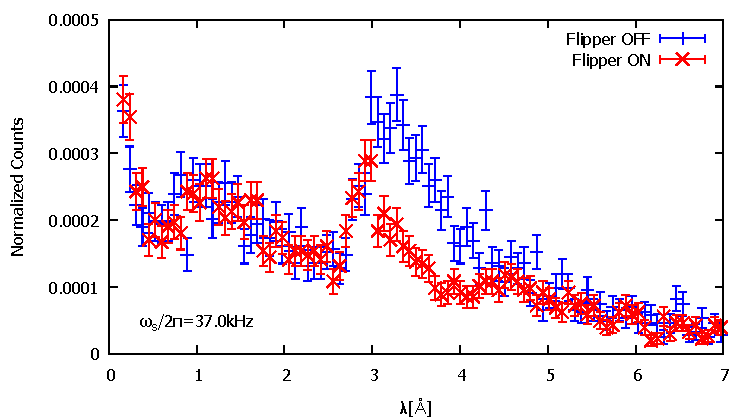
\includegraphics[height=4.3cm]{resonance/analysis/Flipper1_NormalizedCounts_370kHz.pdf}
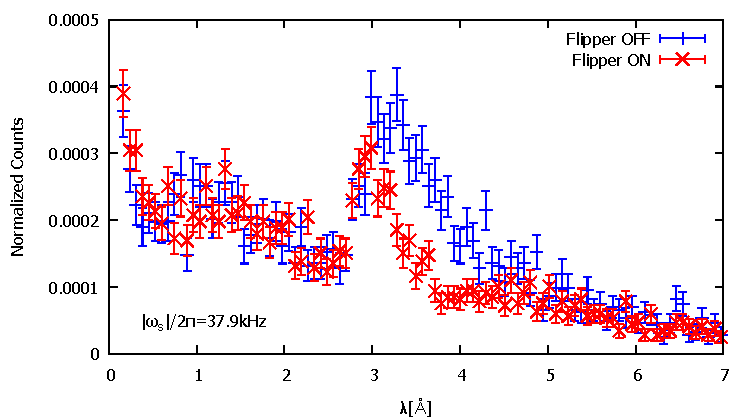
\includegraphics[height=4.3cm]{resonance/analysis/Flipper1_NormalizedCounts_379kHz.pdf}\\
%\end{minipage}
%\begin{minipage}{0.49\hsize}
%\centering
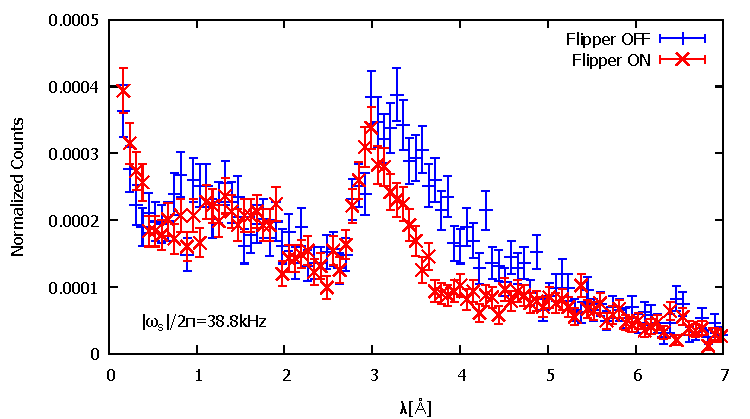
\includegraphics[height=4.3cm]{resonance/analysis/Flipper1_NormalizedCounts_388kHz.pdf}
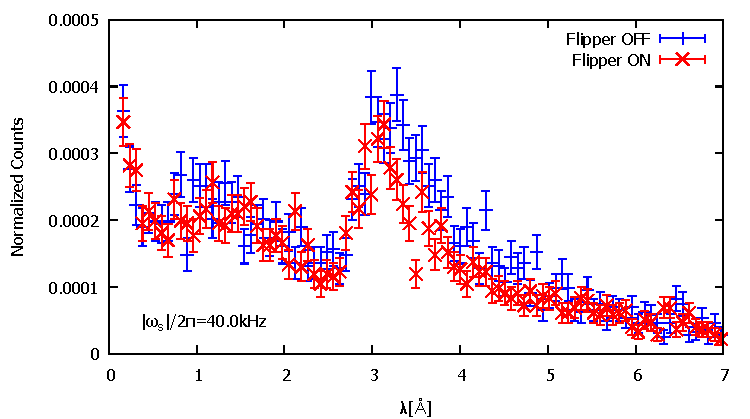
\includegraphics[height=4.3cm]{resonance/analysis/Flipper1_NormalizedCounts_400kHz.pdf}\\
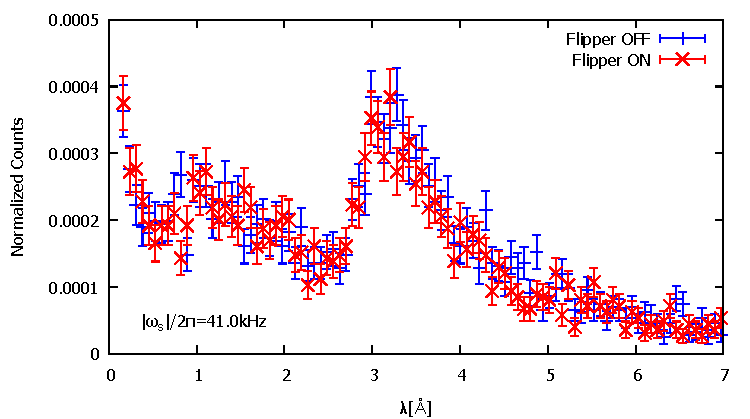
\includegraphics[height=4.3cm]{resonance/analysis/Flipper1_NormalizedCounts_410kHz.pdf}
%\vspace{4.3cm}
%\end{minipage}
\caption{上流フリッパー共鳴実験における規格化粒子数の波長分布}\label{Resonance_fig_Flipper1_NormalizedCounts}
\end{figure}

さらに、図\ref{Resonance_fig_Flipper1_CountsRate}にフリッパーONのときの規格化粒子数をフリッパーOFFのときの規格化粒子数で割ったもの、すなわち上流フリッパーでスピン反転しなかった割合の波長分布を表す。図\ref{Resonance_fig_Flipper1_CountsRate}を見ると、波長$\lambda=$3.0{\AA}から4.5{\AA}あたりで大きく凹んでいることがわかる。
\begin{figure}[h]
%\begin{minipage}{0.49\hsize}
%\centering
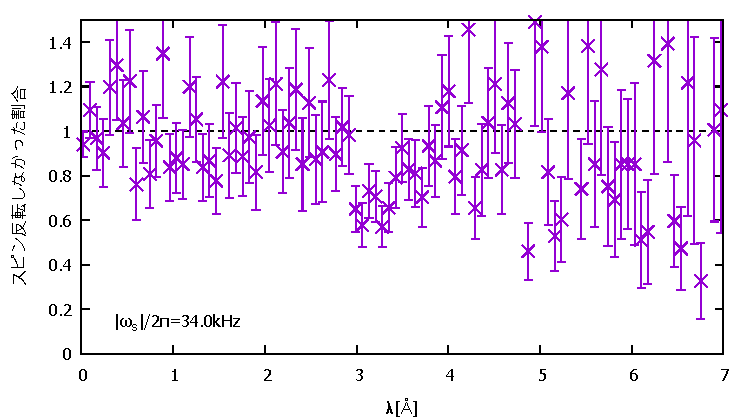
\includegraphics[height=4.3cm]{resonance/analysis/Flipper1_CountsRate_340kHz.pdf}
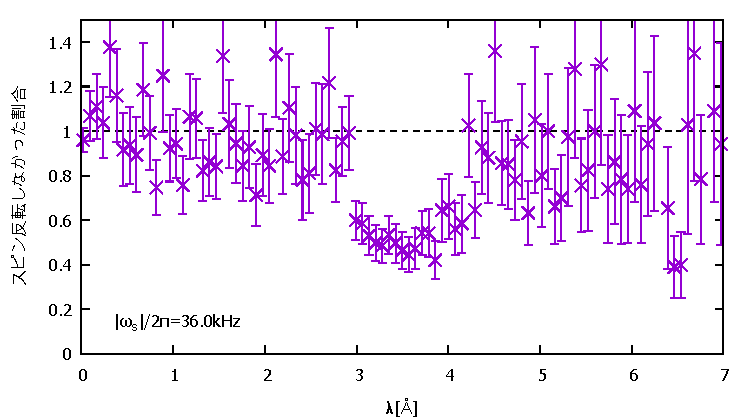
\includegraphics[height=4.3cm]{resonance/analysis/Flipper1_CountsRate_360kHz.pdf}\\
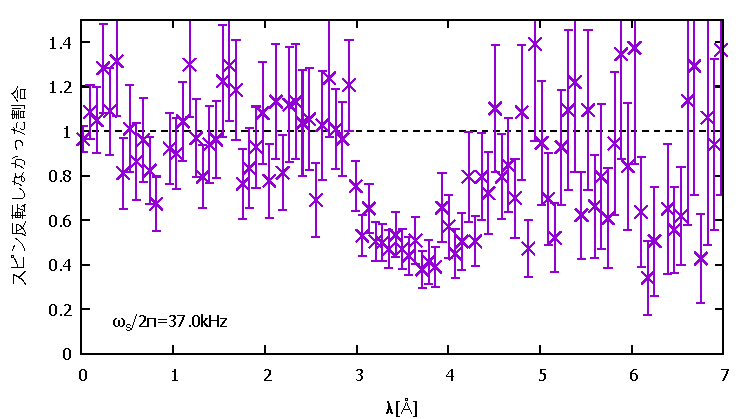
\includegraphics[height=4.3cm]{resonance/analysis/Flipper1_CountsRate_370kHz.pdf}
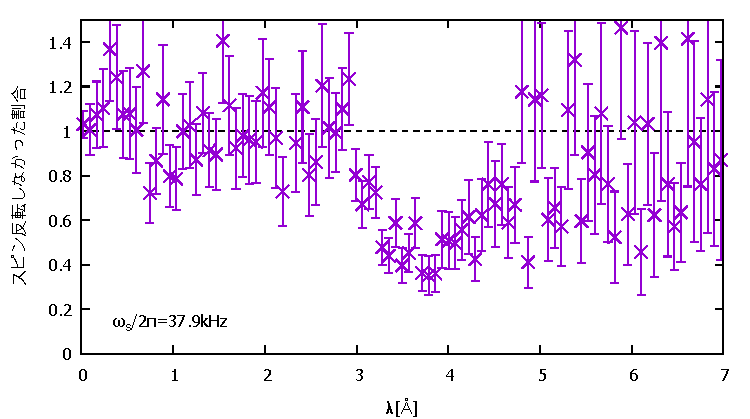
\includegraphics[height=4.3cm]{resonance/analysis/Flipper1_CountsRate_379kHz.pdf}\\
%\end{minipage}
%\begin{minipage}{0.49\hsize}
%\centering
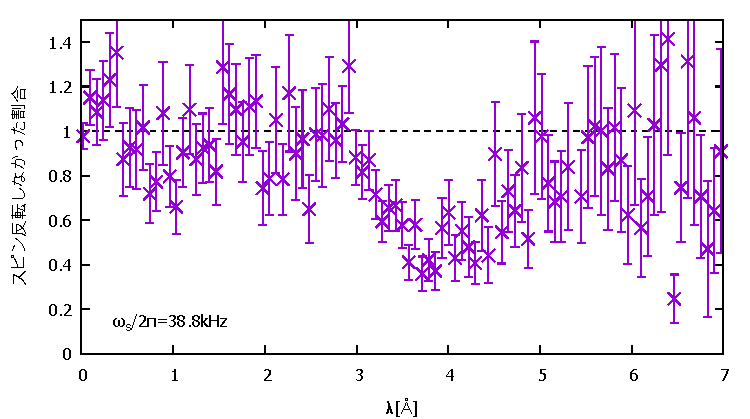
\includegraphics[height=4.3cm]{resonance/analysis/Flipper1_CountsRate_388kHz.pdf}
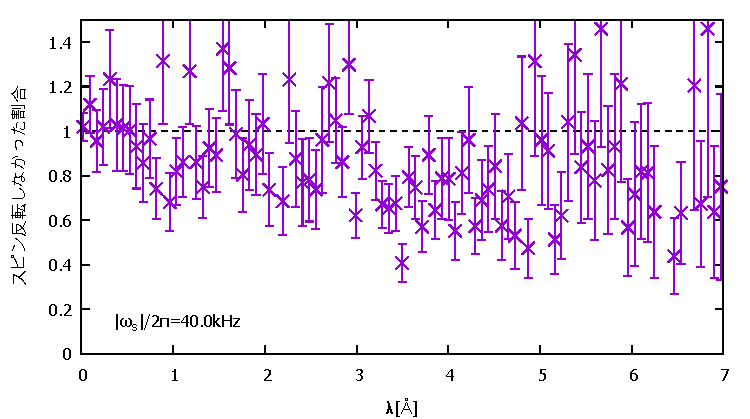
\includegraphics[height=4.3cm]{resonance/analysis/Flipper1_CountsRate_400kHz.pdf}\\
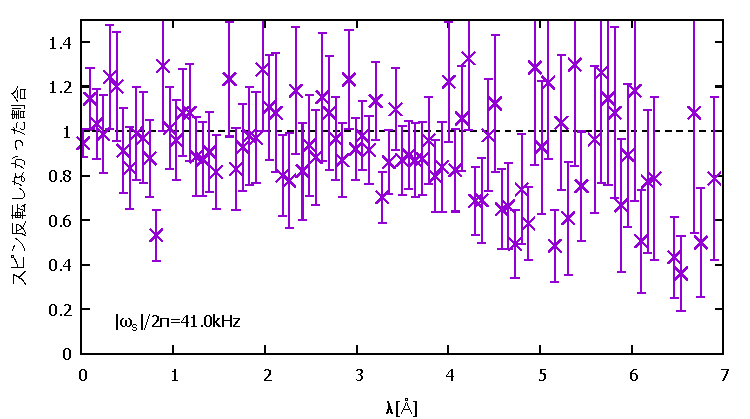
\includegraphics[height=4.3cm]{resonance/analysis/Flipper1_CountsRate_410kHz.pdf}
%\vspace{4.3cm}
%\end{minipage}
\caption{上流フリッパーにおいてスピン反転しなかった割合}\label{Resonance_fig_Flipper1_CountsRate}
\end{figure}

そこで、図\ref{Resonance_fig_Flipper1_NormalizedCounts}の波長領域$\lambda=$3.0{\AA}から4.5{\AA}における規格化粒子数の和を$|\omega_s|/2\pi$を横軸に取って図示すると図\ref{Resonance_fig_Flipper1_Freq}のようになる。2次関数でフィッティングした結果、最もカウントが少なくなる、すなわち共鳴条件(\ref{Resonance_resonance})を満たす$\omega_s$として$|\omega_s|/2\pi=37.17\pm0.03$kHzと決まった。
\begin{comment}
\begin{table}[h]
\centering
\begin{tabular}{c|lllllll}
$|\omega_s|/2\pi$&34.0&36.0&37.0&37.9&38.8&40.0&41.0\\
$3.0{\AA}-4.5{\AA}での規格化粒子数($\times 10^{-4}$)&$17.8\pm0.8$&18.4\pm
\end{comment}
\begin{figure}[h]
\centering
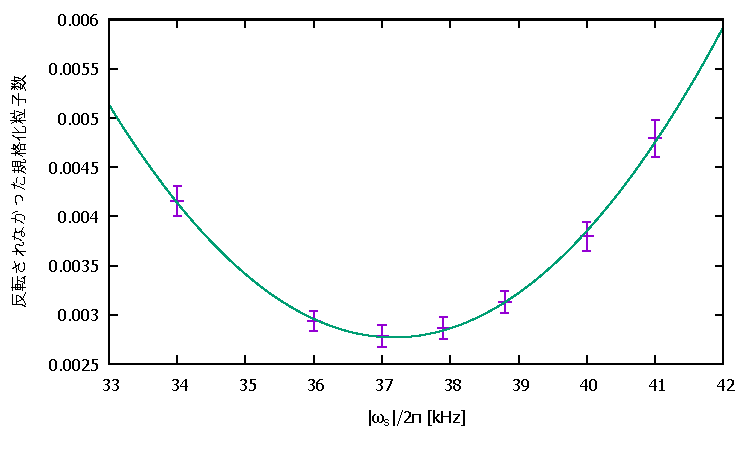
\includegraphics[width=12cm]{resonance/analysis/Flipper1_Freq_30-45r.pdf}
\caption{$|\omega_s|/2\pi$に対する波長$\lambda=$3.0{\AA}から4.5{\AA}における規格化粒子数}\label{Resonance_fig_Flipper1_Freq}
\end{figure}

次に、決まった$\omega_s$と最も近い$|\omega_s|/2\pi=37.0$kHzのときのスピン反転しなかった割合の波長分布(図\ref{Resonance_fig_Flipper1_CountsRate_370fit})から、最も反転しない割合が低い、すなわち最も反転する波長を推定すると、2次関数フィットの結果、$\lambda=3.66\pm0.05${\AA}と求まった。これを速度に直すと$v=1080\pm15$m/sとなり、この速度が$\pi$フリップ条件(\ref{Resonance_piflip})を満たすことから$\omega_{r1}/2\pi=9.0\pm0.1$kHzと計算される。
\begin{figure}[h]
\centering
\includegraphics[width=12cm]{resonance/analysis/Flipper1_CountsRate_370kHz_fit.pdf}
\caption{$|\omega_s|/2\pi$=37.0kHzのときのスピン反転しなかった割合の波長分布}\label{Resonance_fig_Flipper1_CountsRate_370fit}
\end{figure}

\paragraph{下流フリッパーに関する分析}
上流フリッパー同様に下流フリッパーの測定データについても互いに比較するために、測定時間のLiMカウントで規格化を行う。その結果を図\ref{Resonance_fig_Flipper2_NormalizedCounts}に表す。
\begin{figure}[h]
%\begin{minipage}{0.49\hsize}
%\centering
\includegraphics[height=4.3cm]{resonance/analysis/Flipper2_NormalizedCounts_-20A.pdf}
\includegraphics[height=4.3cm]{resonance/analysis/Flipper2_NormalizedCounts_-10A.pdf}\\
\includegraphics[height=4.3cm]{resonance/analysis/Flipper2_NormalizedCounts_-5A.pdf}
\includegraphics[height=4.3cm]{resonance/analysis/Flipper2_NormalizedCounts_0A.pdf}\\
%\end{minipage}
%\begin{minipage}{0.49\hsize}
%\centering
\includegraphics[height=4.3cm]{resonance/analysis/Flipper2_NormalizedCounts_1A.pdf}
\includegraphics[height=4.3cm]{resonance/analysis/Flipper2_NormalizedCounts_3A.pdf}\\
\includegraphics[height=4.3cm]{resonance/analysis/Flipper2_NormalizedCounts_5A.pdf}
\includegraphics[height=4.3cm]{resonance/analysis/Flipper2_NormalizedCounts_10A.pdf}\\
%\vspace{4.3cm}
%\end{minipage}
\includegraphics[height=4.3cm]{resonance/analysis/Flipper2_NormalizedCounts_20A.pdf}
\caption{下流フリッパー共鳴実験における規格化粒子数の波長分布}\label{Resonance_fig_Flipper2_NormalizedCounts}
\end{figure}

さらに、図\ref{Resonance_fig_Flipper2_CountsRate}にフリッパーONのときの規格化粒子数をフリッパーOFFのときの規格化粒子数で割ったもの、すなわち上流フリッパーでスピン反転しなかった割合の波長分布を表す。図\ref{Resonance_fig_Flipper2_CountsRate}を見ると、波長$\lambda=$3.0{\AA}から4.0{\AA}あたりで大きく凹んでいることがわかる。
\begin{figure}[h]
%\begin{minipage}{0.49\hsize}
%\centering
\includegraphics[height=4.3cm]{resonance/analysis/Flipper2_CountsRate_-20A.pdf}
\includegraphics[height=4.3cm]{resonance/analysis/Flipper2_CountsRate_-10A.pdf}\\
\includegraphics[height=4.3cm]{resonance/analysis/Flipper2_CountsRate_-5A.pdf}
\includegraphics[height=4.3cm]{resonance/analysis/Flipper2_CountsRate_0A.pdf}\\
%\end{minipage}
%\begin{minipage}{0.49\hsize}
%\centering
\includegraphics[height=4.3cm]{resonance/analysis/Flipper2_CountsRate_1A.pdf}
\includegraphics[height=4.3cm]{resonance/analysis/Flipper2_CountsRate_3A.pdf}\\
\includegraphics[height=4.3cm]{resonance/analysis/Flipper2_CountsRate_5A.pdf}
\includegraphics[height=4.3cm]{resonance/analysis/Flipper2_CountsRate_10A.pdf}\\
%\vspace{4.3cm}
%\end{minipage}
\includegraphics[height=4.3cm]{resonance/analysis/Flipper2_CountsRate_20A.pdf}
\caption{下流フリッパーにおいてスピン反転しなかった割合}\label{Resonance_fig_Flipper2_CountsRate}
\end{figure}

そこで、図\ref{Resonance_fig_Flipper2_NormalizedCounts}の波長領域$\lambda=$2.7{\AA}から4.2{\AA}における規格化粒子数を数え、$I_c$を横軸として図示すると図\ref{Resonance_fig_Flipper2_Cur}のようになる。2次関数でフィッティングした結果、最もカウントが少なくなる、すなわち共鳴条件(\ref{Resonance_resonance})を満たす$I_c$として$I_c=0.7\pm0.1$Aと決まった。
\begin{figure}[h]
\centering
\includegraphics[width=12cm]{resonance/analysis/Flipper2_Cur_30-40.pdf}
\caption{$I_c$に対する波長$\lambda=$3.0{\AA}から4.0{\AA}における規格化粒子数}\label{Resonance_fig_Flipper2_Cur}
\end{figure}

次に、決まった$I_c$の中心値と最も近い$I_c=0.7$Aのときのスピン反転しなかった割合の波長分布(図\ref{Resonance_fig_Flipper2_CountsRate_7fit})から、最も反転しない割合が低い、すなわち最も反転する波長を推定すると、2次関数フィットの結果、$\lambda=3.40\pm0.03${\AA}と求まった。これを速度に直すと$v=1163\pm10$m/sとなり、この速度が$\pi$フリップ条件(\ref{Resonance_piflip})を満たすことから$\omega_{r2}/2\pi=9.6\pm0.1$kHzと計算される。
\begin{figure}[h]
\centering
\includegraphics[width=12cm]{resonance/analysis/Flipper2_CountsRate_7A_fit.pdf}
\caption{$I_c$=0.7Aのときのスピン反転しなかった割合の波長分布}\label{Resonance_fig_Flipper2_CountsRate_7fit}
\end{figure}

\clearpage
\paragraph{分析まとめ}
以上の分析から各パラメータは次のように決まった。
\begin{table}[h]
\centering
\begin{tabular}{|c|c|} \hline
$|\omega_s|/2\pi$&$37.17\pm0.03$kHz\\ \hline
$I_c$&$0.7\pm0.1$A \\ \hline
$\omega_{r1}/2\pi$&$9.0\pm0.1$kHz \\ \hline
$\omega_{r2}/2\pi$&$9.6\pm0.1$kHz \\ \hline
\end{tabular}
\end{table}

しかし、実験中の粗い解析では$|\omega_s|/2\pi=37.5\pm0.1$kHz,$I_c=0.185\pm0.11$Aと求まったため、実際には以後、
\begin{table}[h]
\centering
\begin{tabular}{|c|c|} \hline
$|\omega_s|/2\pi$&37.5kHz\\ \hline
$I_c$&0.185A \\ \hline
\end{tabular}
\end{table}

\noindent として実験を進めた。このことによる共鳴条件からのずれは最大で$\epsilon/|\omega_z|=$0.1程度であり、十分小さいといえる(図\ref{Resonance_fig_visivility},\ref{Resonance_fig_interference}参照)。


\bibliographystyle{jplain}
\bibliography{bibliography}
\end{document}
